\section{Running Carla}

This section covers details on how to run the CARLA simulator, gather training data, create scenarios and repeat.

\subsection{Setting up VS Code}
To run a jupyter notebook where we can interact with the carla simulator version 0.9.13, we need python version 3.6.9 with carla python api version 0.9.13. Install the carla api version 0.9.13, we need pip 21.3.1.

First, with pyenv, we add the python version
\begin{verbatim}
$ pyenv install 3.6.9$  
\end{verbatim}

Then we create a pyenv environment with the desired python version:
\begin{verbatim}
pyenv virtualenv 3.6.9 carla-env
\end{verbatim}

Then we change directory to the carla PythonAPI directory:
\begin{verbatim}
$cd ~/git/self-driving/carla/PythonAPI
\end{verbatim}
We then create the virtual environment in the PythonAPI directory
\begin{verbatim}
pyenv virtualenv 3.6.9 carla-env
\end{verbatim}

We start the notebook in VS Code, making sure we set the correct pyenv virtual environment. This is done by typing CTRL + SHIFT + P then "kernel", and selecting option "Notebook: Select Notebook Kernel" > "Select Another Kernel..." > "Python Environments..." > "carla-env (Python 3.6.9)"

Before executing cells in the notebook that interact with Carla, make sure Carla is up and running - see next section.

\subsection{Vehicles available in the CARLA Simulator}

\begin{table}[h!]
\centering
\begin{tabular}{|l|l|l|}
\hline
Manufacturer & Model & Blueprint ID \\
\hline
audi & a2 & vehicle.audi.a2 \\
\hline
audi & etron & vehicle.audi.etron \\
\hline
audi & tt & vehicle.audi.tt \\
\hline
bh & crossbike & vehicle.bh.crossbike \\
\hline
bmw & grandtourer & vehicle.bmw.grandtourer \\
\hline
carlamotors & carlacola & vehicle.carlamotors.carlacola \\
\hline
carlamotors & firetruck & vehicle.carlamotors.firetruck \\
\hline
chevrolet & impala & vehicle.chevrolet.impala \\
\hline
citroen & c3 & vehicle.citroen.c3 \\
\hline
diamondback & century & vehicle.diamondback.century \\
\hline
dodge & charger\_2020 & vehicle.dodge.charger\_2020 \\
\hline
dodge & charger\_police & vehicle.dodge.charger\_police \\
\hline
dodge & charger\_police\_2020 & vehicle.dodge.charger\_police\_2020 \\
\hline
ford & ambulance & vehicle.ford.ambulance \\
\hline
ford & crown & vehicle.ford.crown \\
\hline
ford & mustang & vehicle.ford.mustang \\
\hline
gazelle & omafiets & vehicle.gazelle.omafiets \\
\hline
harley-davidson & low\_rider & vehicle.harley-davidson.low\_rider \\
\hline
jeep & wrangler\_rubicon & vehicle.jeep.wrangler\_rubicon \\
\hline
kawasaki & ninja & vehicle.kawasaki.ninja \\
\hline
lincoln & mkz\_2017 & vehicle.lincoln.mkz\_2017 \\
\hline
lincoln & mkz\_2020 & vehicle.lincoln.mkz\_2020 \\
\hline
mercedes & coupe & vehicle.mercedes.coupe \\
\hline
mercedes & coupe\_2020 & vehicle.mercedes.coupe\_2020 \\
\hline
mercedes & sprinter & vehicle.mercedes.sprinter \\
\hline
micro & microlino & vehicle.micro.microlino \\
\hline
mini & cooper\_s & vehicle.mini.cooper\_s \\
\hline
mini & cooper\_s\_2021 & vehicle.mini.cooper\_s\_2021 \\
\hline
nissan & micra & vehicle.nissan.micra \\
\hline
nissan & patrol & vehicle.nissan.patrol \\
\hline
nissan & patrol\_2021 & vehicle.nissan.patrol\_2021 \\
\hline
seat & leon & vehicle.seat.leon \\
\hline
tesla & cybertruck & vehicle.tesla.cybertruck \\
\hline
tesla & model3 & vehicle.tesla.model3 \\
\hline
toyota & prius & vehicle.toyota.prius \\
\hline
vespa & zx125 & vehicle.vespa.zx125 \\
\hline
volkswagen & t2 & vehicle.volkswagen.t2 \\
\hline
volkswagen & t2\_2021 & vehicle.volkswagen.t2\_2021 \\
\hline
yamaha & yzf & vehicle.yamaha.yzf \\
\hline
\end{tabular}
\caption{Available vehicles in CARLA simulator with their blueprint IDs}
\label{tab:carla-vehicles}
\end{table}

\subsection{CARLA Transform System}

\begin{figure}[h!]
    \centering
    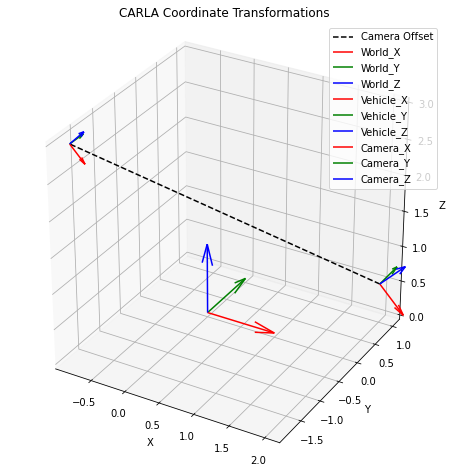
\includegraphics[width=0.75\textwidth]{Figures/Methods/Carla_transformations.png}
    \caption{Visualization of CARLA coordinate transformations.}
    % \caption{CARLA simulator with Town 10 loaded, plus dynamic weather at 0.05 speed, where sun is currently below the horizon (altitude -19.33).}    
    \label{fig:Carla_transformations}
\end{figure}

Figure \ref{fig:Carla_transformations} shows three coordinate frames: world coordinates (largest axes, at origin), vehicle coordinates (medium axes, positioned at (2,1,0.5) with 45 degree yaw), and camera coordinates (smallest axes). The dashed line represents the camera offset vector (-4,0,2.5) relative to the vehicle position. Each coordinate frame is represented by its three principal axes: X (red), Y (green), and Z (blue), illustrating the spatial relationships and rotations between the different reference frames in the simulation.


\subsubsection{Coordinate System Fundamentals}
CARLA utilizes a right-handed coordinate system where:
\begin{itemize}
    \item The X-axis represents the forward direction
    \item The Y-axis represents the right direction
    \item The Z-axis represents the upward direction
\end{itemize}

\subsubsection{Transform Components}
A transform in CARLA consists of two primary components:

\paragraph{Location} Defined by a vector $\vec{p} = (x, y, z)$ representing a point in 3D space.

\paragraph{Rotation} Represented by Euler angles $(\phi, \theta, \psi)$ where:
\begin{itemize}
    \item Pitch ($\phi$): rotation around Y-axis
    \item Yaw ($\theta$): rotation around Z-axis
    \item Roll ($\psi$): rotation around X-axis
\end{itemize}

\subsubsection{Mathematical Framework}
The transformation of a point from local to world coordinates involves two steps:

\paragraph{1. Rotation Matrix}
The combined rotation matrix $R$ is composed of individual rotations:
\begin{equation}
R = R_z(\psi)R_y(\theta)R_x(\phi)
\end{equation}

Where:
\begin{equation}
R_x(\phi) = \begin{pmatrix}
1 & 0 & 0 \\
0 & \cos(\phi) & -\sin(\phi) \\
0 & \sin(\phi) & \cos(\phi)
\end{pmatrix}
\end{equation}

\begin{equation}
R_y(\theta) = \begin{pmatrix}
\cos(\theta) & 0 & \sin(\theta) \\
0 & 1 & 0 \\
-\sin(\theta) & 0 & \cos(\theta)
\end{pmatrix}
\end{equation}

\begin{equation}
R_z(\psi) = \begin{pmatrix}
\cos(\psi) & -\sin(\psi) & 0 \\
\sin(\psi) & \cos(\psi) & 0 \\
0 & 0 & 1
\end{pmatrix}
\end{equation}

\paragraph{2. Complete Transform}
The complete transformation of a point $\vec{p}_{local}$ to world coordinates $\vec{p}_{world}$ is given by:
\begin{equation}
\vec{p}_{world} = R\vec{p}_{local} + \vec{t}
\end{equation}

Where $\vec{t}$ is the translation vector representing the origin of the local coordinate system in world coordinates.

\subsubsection{Application in CARLA}
In CARLA, this transformation is encapsulated in the \texttt{transform()} method. For example, when positioning a spectator camera:
\begin{equation}
\vec{p}_{camera} = T_{vehicle}(\vec{p}_{relative})
\end{equation}

Where:
\begin{itemize}
    \item $\vec{p}_{relative}$ is the desired camera position relative to the vehicle (e.g., (-4, 0, 2.5))
    \item $T_{vehicle}$ is the vehicle's transform in world coordinates
    \item $\vec{p}_{camera}$ is the resulting camera position in world coordinates
\end{itemize}

\subsubsection{Practical Implications}
This transform system enables:
\begin{itemize}
    \item Precise positioning of sensors relative to vehicles
    \item Accurate conversion between local and global coordinates
    \item Proper orientation of vehicles and objects in the simulation
    \item Consistent reference frame transformations for perception and control algorithms
\end{itemize}

\subsubsection{Example}

\begin{figure}[h!]
    \centering
    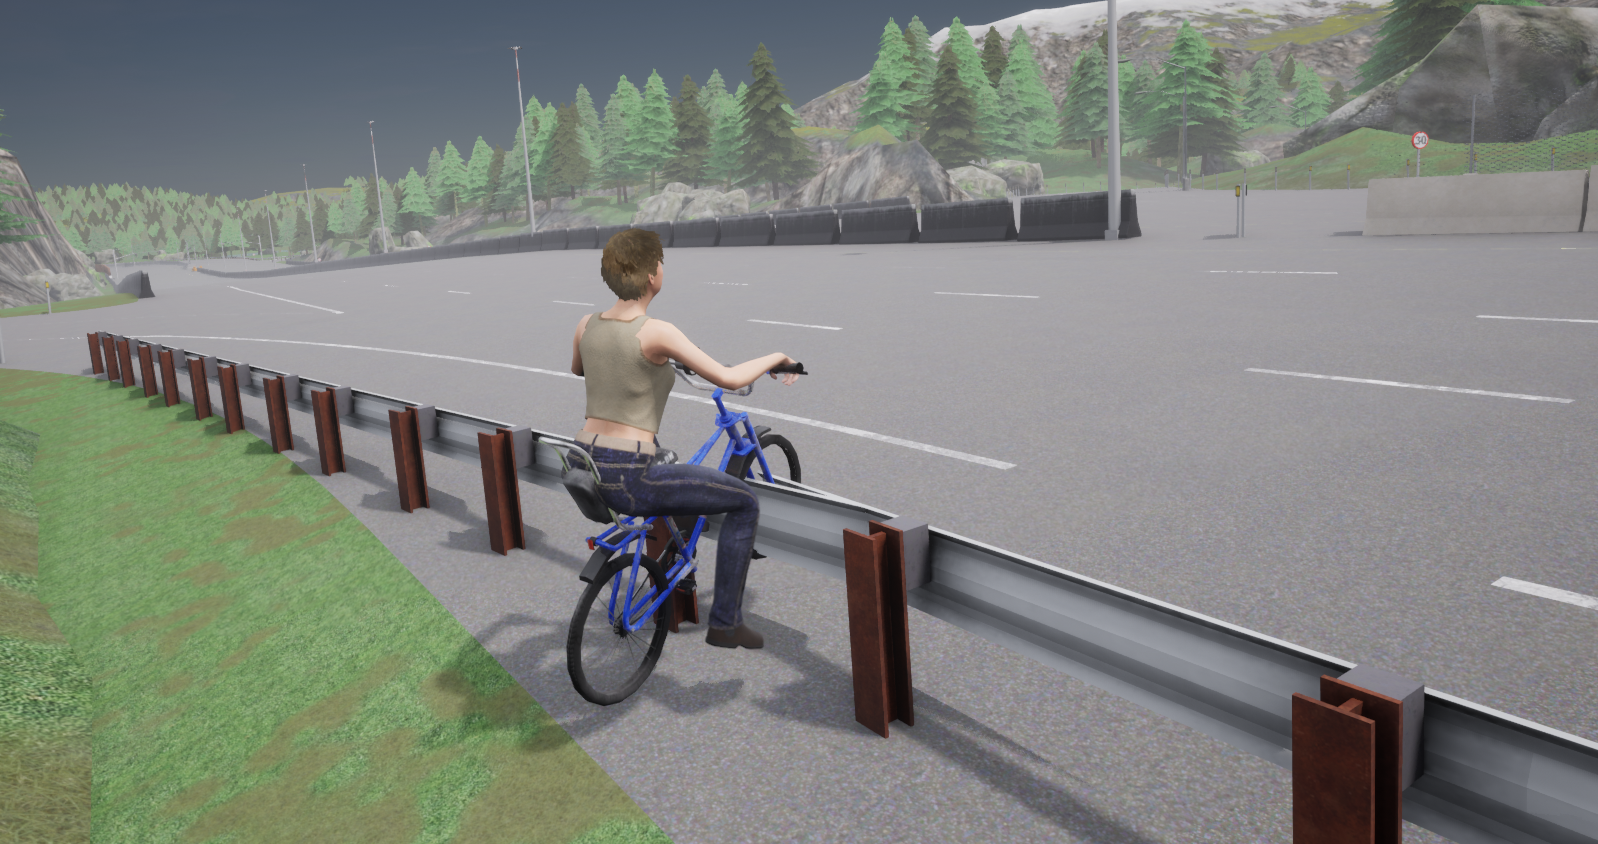
\includegraphics[width=0.50\textwidth]{Figures/Methods/Carla_stuck_cyclist.png}
    \caption{Determining coordinate information for a CARLA vehicle.}
    % \caption{CARLA simulator with Town 10 loaded, plus dynamic weather at 0.05 speed, where sun is currently below the horizon (altitude -19.33).}    
    \label{fig:Carla_stuck_cyclist}
\end{figure}

Figure \ref{fig:Carla_stuck_cyclist} shows a cyclist that, having been set to autopilot, got stuck on a guard rail. The orientation of the vehicle can be determined in code:

\begin{verbatim}
# Get the transform
transform = vehicle.get_transform()

# Print full transform
print("\nFull transform:")
print(transform)

# Print location details
print("\nLocation details:")
print(f"x: {transform.location.x}")
print(f"y: {transform.location.y}")
print(f"z: {transform.location.z}")


\end{verbatim}

\subsection{Starting CARLA}

We start CARLA by typing on the prompt of a computer with CARLA installed, note operating system is Ubuntu 18.04:

%% TODO installation was done with sudo apt-get install
%% Last stable version at the time was 0.9.13
%% Stable Ubuntu version is 18.04 which is no longer supported
%% by Canonical

\begin{verbatim}
daniel@simbox:/opt/carla-simulator$ ./CarlaUE4.sh 
4.26.2-0+++UE4+Release-4.26 522 0
Disabling core dumps.
\end{verbatim}

\subsection{Adding cars, pedestrians and changeable weather}

The CARLA repository has examples of using the Python API to generate traffic and changing weather. In the example below, 20 cars and 60 pedestrians are added:

\begin{verbatim}
daniel@simbox:/opt/carla-simulator/PythonAPI/examples$ python \\
generate_traffic.py -n 20 -w 60
ERROR: Spawn failed because of collision at spawn position
ERROR: Spawn failed because of collision at spawn position
ERROR: Spawn failed because of collision at spawn position
ERROR: Spawn failed because of collision at spawn position
spawned 20 vehicles and 56 walkers, press Ctrl+C to exit.
\end{verbatim}

% \begin{figure}[h]
%     \centering
%     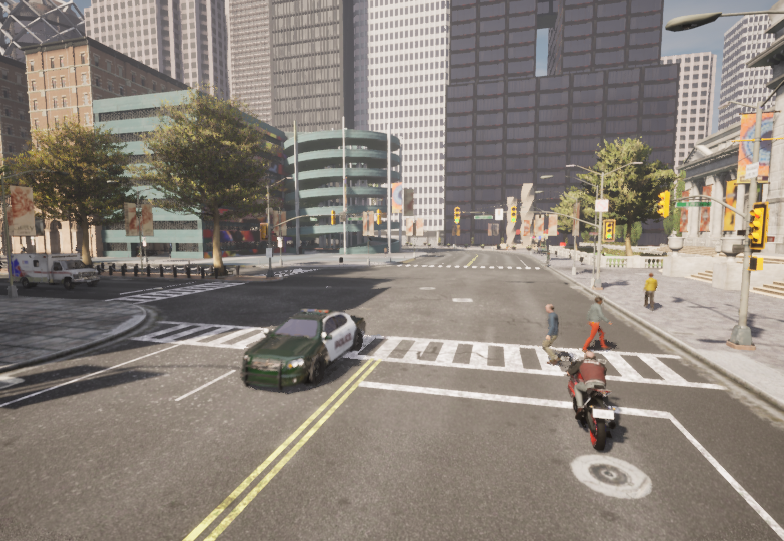
\includegraphics[width=0.99\textwidth]{Figures/Methods/CARLA_20_Cars_60_pedestrians.png}
%     \caption{CARLA simulator with Town 10 loaded, plus 20 cars and 60 pedestrians.}
%     \label{fig:CARLA_20_Cars_60_pedestrians}
% \end{figure}

In the example below, changing weather is included. The position of the sun in the sky follows the 

\begin{verbatim}
daniel@simbox:/opt/carla-simulator/PythonAPI/examples$ python \\ 
dynamic_weather.py --speed 0.05 \\
Sun(alt: -19.33, azm: 300.30) Storm(clouds=0%, rain=0%, wind=5%)           
\end{verbatim}

% \begin{figure}[h]
%     \centering
%     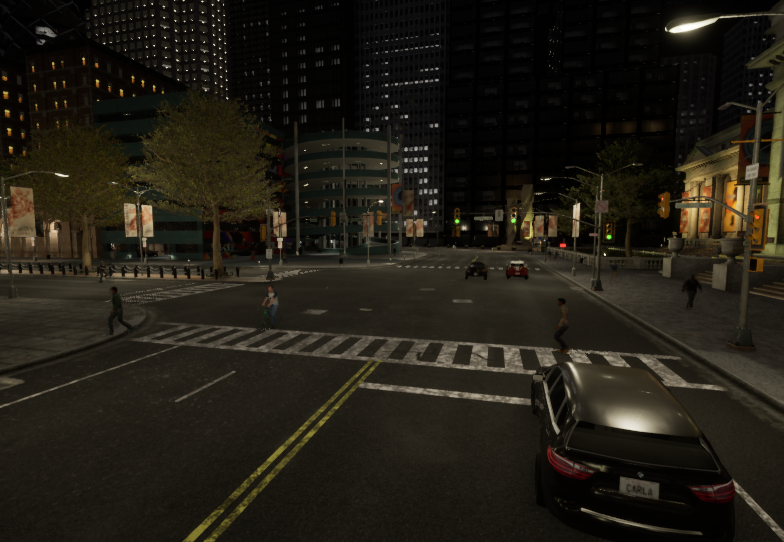
\includegraphics[width=0.99\textwidth]{Figures/Methods/CARLA_Dynamic_Weather_speed_0.05.png}
%     \caption{CARLA simulator with Town 10 loaded, plus dynamic weather at 0.05 speed, where sun is currently below the horizon (altitude -19.33).}
%     \label{fig:CARLA_Dynamic_Weather_speed_0.05}
% \end{figure}

\begin{figure}[h]
    \centering
    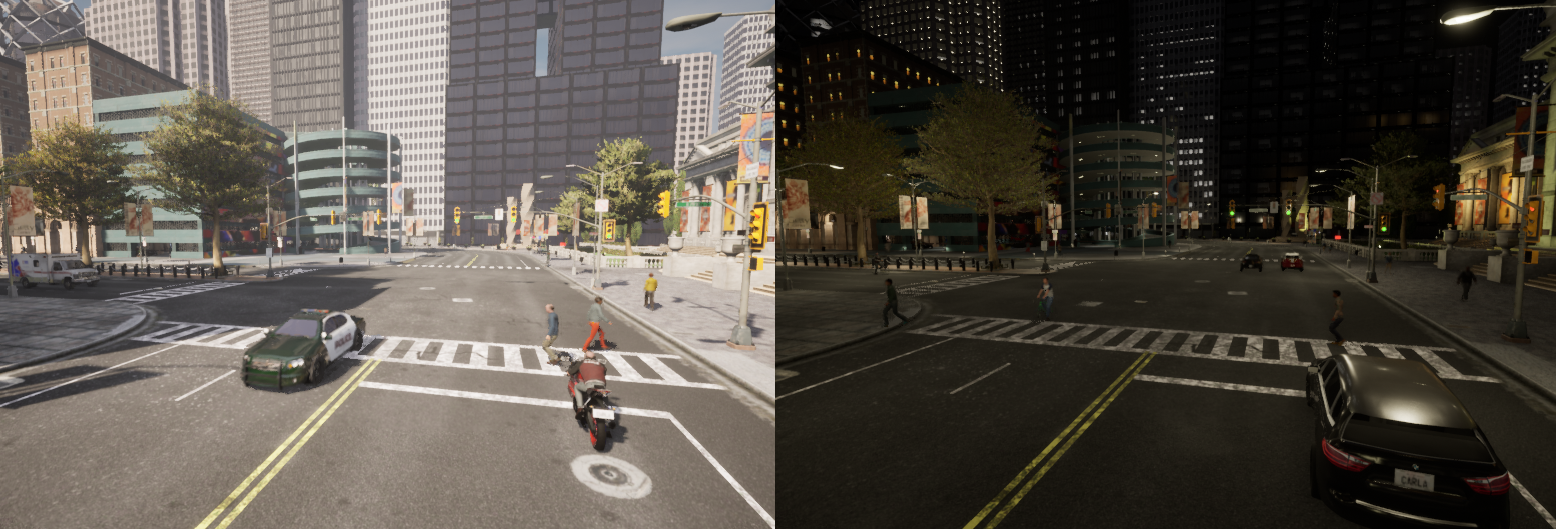
\includegraphics[width=0.99\textwidth]{Figures/Methods/CARLA_Traffic_Weather_Combined.png}
    \caption{CARLA simulator with Town 10 loaded, plus 20 vehicles and 60 pedestrians on the left, and dynamic weather at 0.05 speed added on the right, where sun is, at the time screen was captured, below the horizon (altitude -19.33).}
    \label{fig:CARLA_Traffic_Weather_Combined}
\end{figure}

\subsection{Running Jupyter Notebooks in the Selfdrive repository}

The Selfdrive repository is a collection of Jupyter Notebooks that interact with Carla via the iPython web interface. In the setup used for the work presented here, the notebooks are run with VS Code Insiders \cite{todo}. At the time of writing, both the CARLA install and pip carla versions must be the same (0.9.13). To satisfy the condition, python 3.6.9 is used, as both run with the version. In VS Code the same version must be selected.

\subsection{Maps}

Cityscapes are defined in Carla as maps. Available maps for a Carla version can be found in:
\begin{verbatim}
/opt/carla-simulator/CarlaUE4/Content/Carla/Maps/    
\end{verbatim}

The maps available for version 0.9.13 are:
% ls /opt/carla-simulator/CarlaUE4/Content/Carla/Maps/*.umap | cut -d '/' -f 8
\begin{verbatim}
OpenDriveMap.umap
Town01_Opt.umap
Town01.umap
Town02_Opt.umap
Town02.umap
Town03_Opt.umap
Town03.umap
Town04_Opt.umap
Town04.umap
Town05_Opt.umap
Town05.umap
Town06_Opt.umap
Town06.umap
Town07_Opt.umap
Town07.umap
Town10HD_Opt.umap
Town10HD.umap
\end{verbatim}

\begin{table}[h]
\centering
\begin{tabular}{lll}
\hline
\textbf{Axis} & \textbf{Direction} & \textbf{Effect} \\
\hline
X (Pitch) & Negative (-) & Tilt Down \\
          & Positive (+) & Tilt Up \\
\hline
Y (Yaw)   & 0°   & Forward \\
          & 90°  & Right \\
          & -90° & Left \\
          & 180° & Backward \\
\hline
Z (Roll)  & Negative (-) & Counter-clockwise tilt \\
          & Positive (+) & Clockwise tilt \\
\hline
\end{tabular}

\vspace{10pt}

\begin{tabular}{ll}
\hline
\textbf{View} & \textbf{(Pitch, Yaw, Roll)} \\
\hline
Back view  & (0°, 0°, 0°) \\
Front view & (0°, 180°, 0°) \\
Right view & (0°, 90°, 0°) \\
Left view  & (0°, -90°, 0°) \\
\hline
\end{tabular}
\caption{Camera Rotation Reference}
\label{cam_rotation_reference}
\end{table}

Key points to note in Table \ref{cam_rotation_reference}:
\begin{enumerate}
    \item Pitch (X-axis) controls vertical tilt, allowing the camera to look up or down relative to the horizon
    \item Yaw (Y-axis) handles horizontal rotation, enabling full 360-degree coverage around the vertical axis
    \item Roll (Z-axis) affects camera tilt around viewing axis, creating Dutch angles and perspective shifts
    \item Standard views maintain 0° pitch and roll for level viewing, ensuring stable and natural perspectives
    \item Yaw values follow right-hand rule: positive clockwise when viewed from above, providing consistent directional reference
\end{enumerate}

\subsection{Collecting Training Data}

We use map Town04 to collect data around a figure of eight, where the self-driving car will need to steer straight, left and right. Figure \ref{fig:Town04FigureOfEight}. The image is taken from coordinates The red segments are representations internal to Carla of roads, where each segment represents a road ID, where x = -56.26, y = 4.20, z = 554.04),  pitch(x) = -87.06, yaw(y) = 54.52 and row(z) =  0, meaning the spectator is placed at x and y offsets of the origin and 554 units above the map, while the view is tilted down (pitch) almost ninety degrees and turned right/clockwise (yaw) 55 degrees. 

%% Figure generated by https://github.com/dsikar/carla-driver-data/scripts/18-town04-figure-of-8-draft.ipynb
%% Commit: c5529ba

\begin{figure}[h]
    \centering
    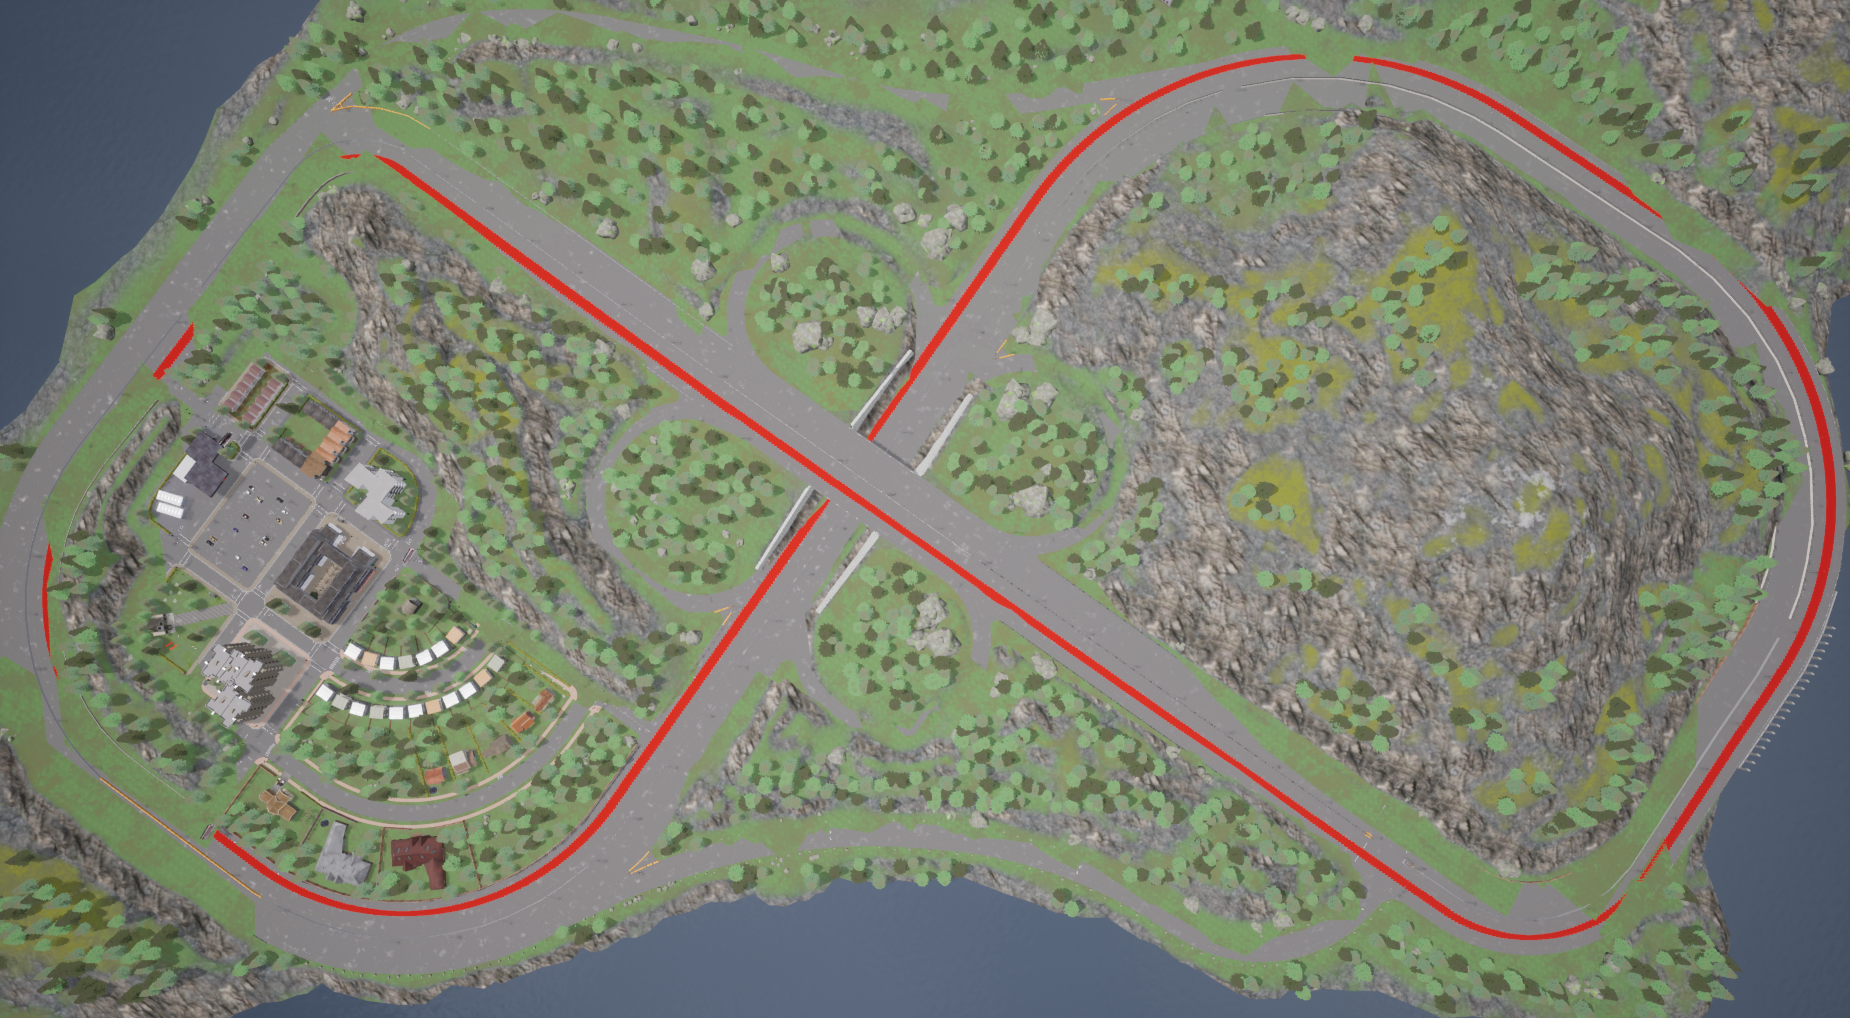
\includegraphics[width=0.99\textwidth]{Figures/Methods/Town04FigureOfEight.png}
    \caption{Town04 in Carla showing figure of eight peripheral road}
    \label{fig:Town04FigureOfEight}
\end{figure}

The Carla \textit{world} object represents a map e.g Town04 and contains \textit{waypoints} metadata that provide geometrical anchors for orientation and navigation, making it possible for a vehicle to follow a route based on these metadata. Figure \ref{fig:Town04Waypoints} shows a detail of Town04 with all waypoints displayed at 1 metre intervals. Such interval generates 33670 waypoints on the map. Waypoints, having a \textit{transform} property with location (translation) and rotation, can also be used to spawn vehicles in the desired orientation, as well as generate steering adjustments for a vehicle in motion, by aligning transform vectors between vehicle and nearest forward waypoint along a desired route.

%% Waypoint properties
% {'__class__': carla.libcarla.Waypoint,
%  '__delattr__': <method-wrapper '__delattr__' of Waypoint object at 0x7ff84068c0e0>,
%  '__dict__': {},
%  '__dir__': <function Waypoint.__dir__>,
%  '__doc__': None,
%  '__eq__': <method-wrapper '__eq__' of Waypoint object at 0x7ff84068c0e0>,
%  '__format__': <function Waypoint.__format__>,
%  '__ge__': <method-wrapper '__ge__' of Waypoint object at 0x7ff84068c0e0>,
%  '__getattribute__': <method-wrapper '__getattribute__' of Waypoint object at 0x7ff84068c0e0>,
%  '__gt__': <method-wrapper '__gt__' of Waypoint object at 0x7ff84068c0e0>,
%  '__hash__': <method-wrapper '__hash__' of Waypoint object at 0x7ff84068c0e0>,
%  '__init__': <function __init__>,
%  '__init_subclass__': <function Waypoint.__init_subclass__>,
%  '__le__': <method-wrapper '__le__' of Waypoint object at 0x7ff84068c0e0>,
%  '__lt__': <method-wrapper '__lt__' of Waypoint object at 0x7ff84068c0e0>,
%  '__module__': 'carla.libcarla',
%  '__ne__': <method-wrapper '__ne__' of Waypoint object at 0x7ff84068c0e0>,
%  '__new__': <function instance.__new__(*args, **kwargs)>,
%  '__reduce__': <bound method <unnamed Boost.Python function> of <carla.libcarla.Waypoint object at 0x7ff84068c0e0>>,
%  '__reduce_ex__': <function Waypoint.__reduce_ex__>,
%  '__repr__': <method-wrapper '__repr__' of Waypoint object at 0x7ff84068c0e0>,
%  '__setattr__': <method-wrapper '__setattr__' of Waypoint object at 0x7ff84068c0e0>,
%  '__sizeof__': <function Waypoint.__sizeof__>,
%  '__str__': <bound method __str__ of <carla.libcarla.Waypoint object at 0x7ff84068c0e0>>,
%  '__subclasshook__': <function Waypoint.__subclasshook__>,
%  '__weakref__': None,
%  'get_junction': <bound method get_junction of <carla.libcarla.Waypoint object at 0x7ff84068c0e0>>,
%  'get_landmarks': <bound method get_landmarks of <carla.libcarla.Waypoint object at 0x7ff84068c0e0>>,
%  'get_landmarks_of_type': <bound method get_landmarks_of_type of <carla.libcarla.Waypoint object at 0x7ff84068c0e0>>,
%  'get_left_lane': <bound method get_left_lane of <carla.libcarla.Waypoint object at 0x7ff84068c0e0>>,
%  'get_right_lane': <bound method get_right_lane of <carla.libcarla.Waypoint object at 0x7ff84068c0e0>>,
%  'id': 16652337276301294135,
%  'is_intersection': True,
%  'is_junction': True,
%  'junction_id': 1368,
%  'lane_change': carla.libcarla.LaneChange.NONE,
%  'lane_id': -1,
%  'lane_type': carla.libcarla.LaneType.Driving,
%  'lane_width': 3.5,
%  'left_lane_marking': <carla.libcarla.LaneMarking at 0x7ff8407003a0>,
%  'next': <bound method next of <carla.libcarla.Waypoint object at 0x7ff84068c0e0>>,
%  'next_until_lane_end': <bound method next_until_lane_end of <carla.libcarla.Waypoint object at 0x7ff84068c0e0>>,
%  'previous': <bound method previous of <carla.libcarla.Waypoint object at 0x7ff84068c0e0>>,
%  'previous_until_lane_start': <bound method previous_until_lane_start of <carla.libcarla.Waypoint object at 0x7ff84068c0e0>>,
%  'right_lane_marking': <carla.libcarla.LaneMarking at 0x7ff840700608>,
%  'road_id': 1450,
%  's': 44.0,
%  'section_id': 0,
%  'transform': <carla.libcarla.Transform at 0x7ff853a24e10>}

\begin{figure}[h]
    \centering
    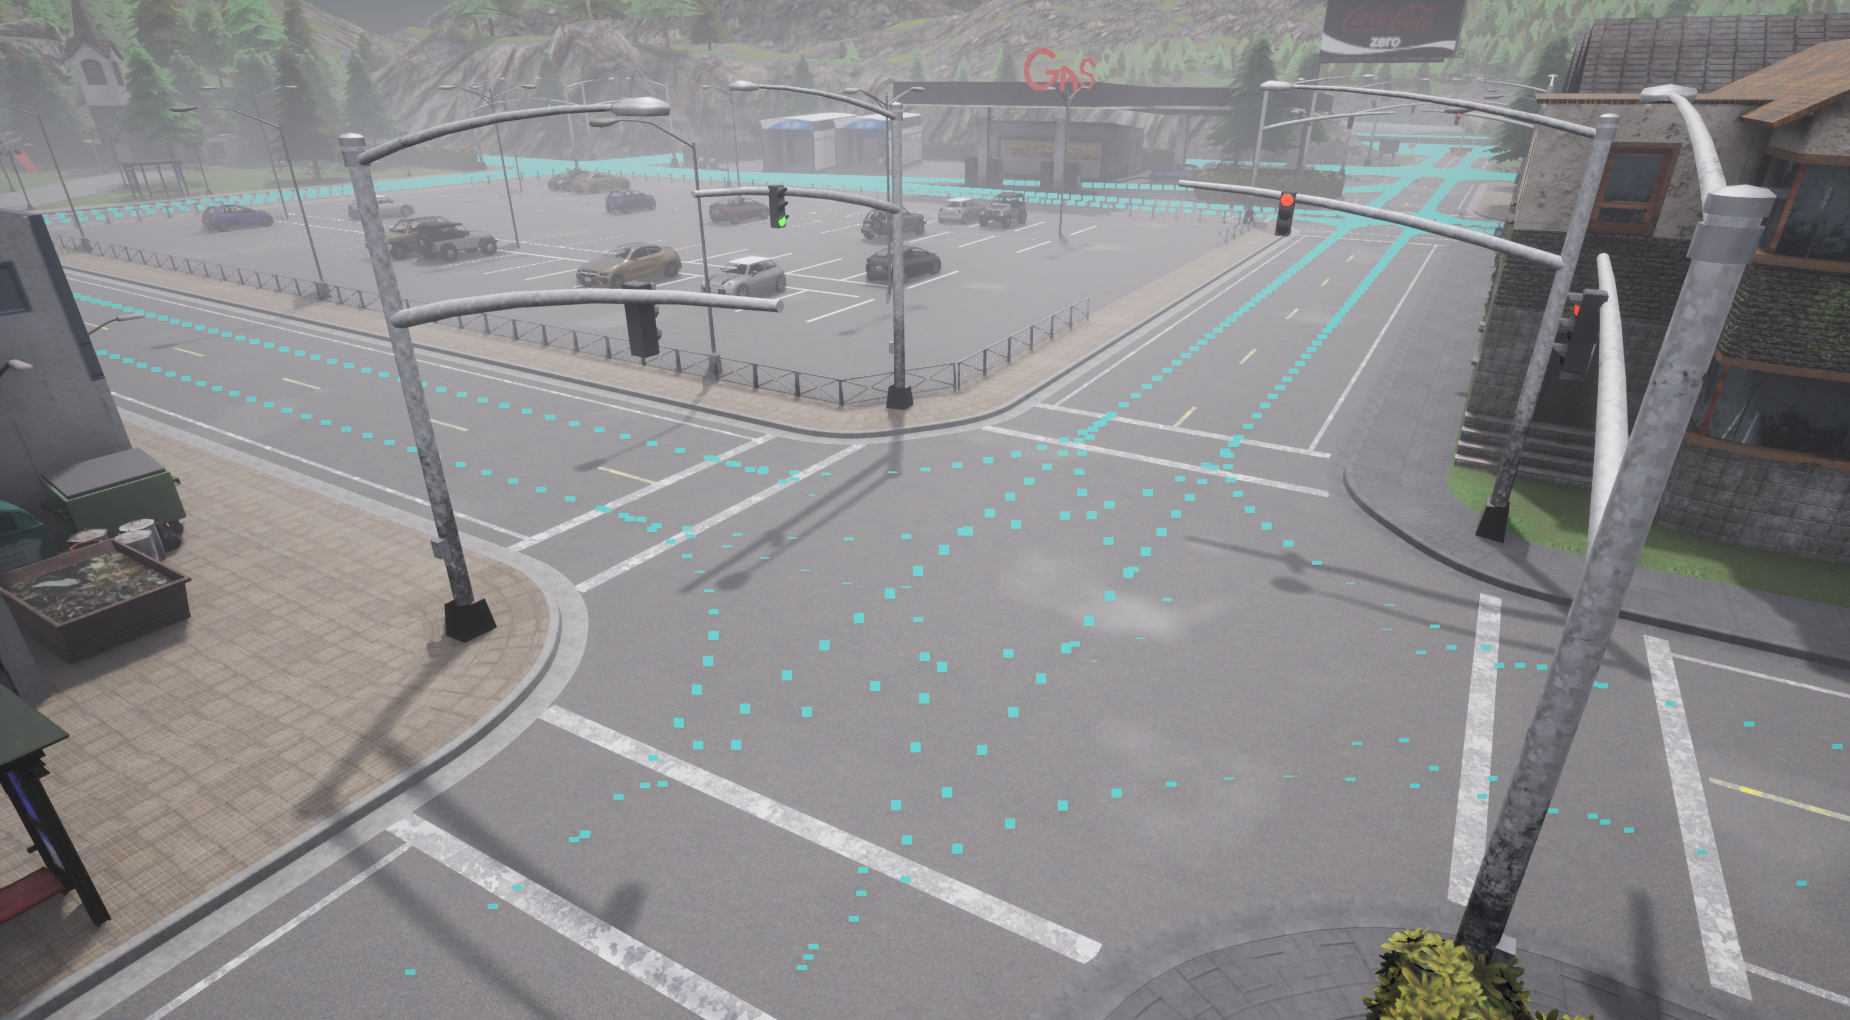
\includegraphics[width=0.99\textwidth]{Figures/Methods/Town04Waypoints.png}
    \caption{Town04 Carla map showing a detail of the town centre with all waypoints spawend at a distance of 1 unit}
    \label{fig:Town04Waypoints}
\end{figure}

To capture all waypoints of the figure-of-eight route, the road\_id property is extracted from all waypoints, then each road\_id examined in turn to verify which ones have 4 lanes using property lane\_id. Note, the outer road is the only one on Town04 that contains 4 lanes. Then all waypoints that have property lane\_id = -3, that is, the second lane from right to left. We avoid the furthest lane to the left (lane\_id = 4) because it contains exits, that do not allow for continuous driving. The final selection contains the route that is used to collect our training data.

\subsection{Spawn Points}

Spawn points in CARLA are defined through the \texttt{carla.Transform} class, representing transformations that combine location and rotation in 3D space. The class implements transformation without scaling and consists of two primary components:

\begin{itemize}
    \item \textbf{Location} (\texttt{carla.Location}): Defines coordinates in the simulation space
    \item \textbf{Rotation} (\texttt{carla.Rotation}): Specifies orientation using pitch, yaw, and roll (in degrees)
\end{itemize}

The class provides several methods for coordinate manipulation:

\begin{lstlisting}[language=Python]
# Initialization
transform = carla.Transform(location, rotation)

# Coordinate transformations
global_point = transform.transform(local_point)
rotated_vector = transform.transform_vector(velocity)
\end{lstlisting}

Direction vectors can be obtained through:
\begin{itemize}
    \item \texttt{get\_forward\_vector()}: Returns forward direction
    \item \texttt{get\_right\_vector()}: Returns right direction
    \item \texttt{get\_up\_vector()}: Returns up direction
\end{itemize}

For matrix operations, the class provides:
\begin{itemize}
    \item \texttt{get\_matrix()}: Returns 4x4 transformation matrix
    \item \texttt{get\_inverse\_matrix()}: Returns inverse transformation matrix
\end{itemize}

Example usage for vehicle spawning:
\begin{lstlisting}[language=Python]
spawn_point = carla.Transform(
    carla.Location(x=10.0, y=0.0, z=2.0),
    carla.Rotation(pitch=0.0, yaw=90.0, roll=0.0)
)
vehicle = world.spawn_actor(vehicle_bp, spawn_point)
\end{lstlisting}

\begin{figure}[h]
    \centering
    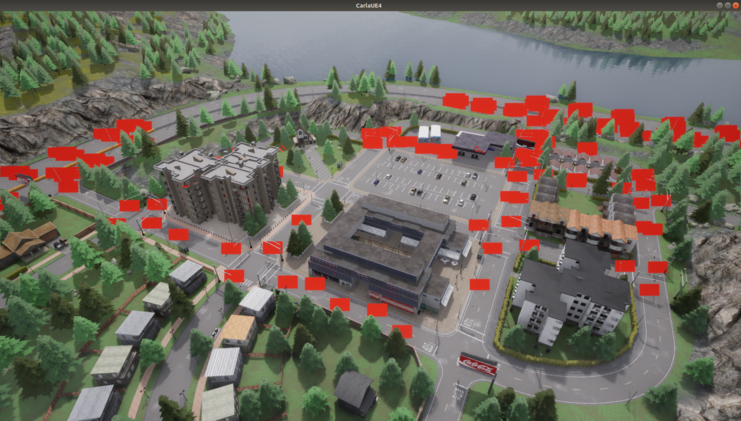
\includegraphics[width=0.99\textwidth]{Figures/Methods/CarlaSpawnPointsTown04_40pc.png}
    \caption{Town04 in Carla simulator with spawn points markers}
    \label{fig:CarlaSpawnPointsTown04_40pc}
\end{figure}

Figure \ref{fig:CarlaSpawnPointsTown04_40pc} shows highlighted with red markers the spawn points, locations where vehicle objects are initially placed by default on a map. A spawn point is essentially a Transform method of a carla object, and store location, rotation and matrix transform information, such that can be retrieved from and object.

\subsection{Analysis of Transform Objects: Directional Vectors and Matrices}

The Transform object from spawn point 145 in Town04 provides insight into the spatial configuration through its vector and matrix representations. The directional vectors indicate:

\begin{itemize}
    \item Forward vector (0.72, -0.35, -0.60) shows significant forward tilt with downward orientation
    \item Right vector (0.44, 0.90, 0.00) indicates rightward bias with minimal vertical component
    \item Up vector (0.54, -0.27, 0.80) confirms upward orientation with slight backward tilt
\end{itemize}

The transformation matrix represents the complete spatial transformation:
\begin{equation*}
\begin{bmatrix}
0.72 & 0.44 & 0.54 & 135.89 \\
-0.35 & 0.90 & -0.27 & -168.36 \\
-0.60 & 0.00 & 0.80 & 93.85 \\
0.00 & 0.00 & 0.00 & 1.00
\end{bmatrix}
\end{equation*}

Here, the rightmost column (135.89, -168.36, 93.85, 1.00) represents the translation component, indicating the spawn point's position in world coordinates. The 3x3 submatrix in the upper left defines the rotation, constructed from the directional vectors.

The inverse matrix facilitates transformation from world to local coordinates, essential for relative positioning calculations. The symmetry between certain elements in the transformation and inverse matrices validates the mathematical consistency of the Transform object's representation.

\subsection{Vehicle Steering Control Mapping}

The relationship between steering control inputs and physical steering angles demonstrates a linear mapping constrained by the vehicle's maximum steering angle. As shown in Table \ref{tab:steering_range}, the control values range from -1.0 to 1.0, corresponding to steering angles from -70° to 70° for the default vehicle model. This mapping can be expressed as:

\begin{equation}
\theta = c \cdot \theta_{max}
\end{equation}

where $\theta$ is the resulting steering angle, $c$ is the control input value ($-1 \leq c \leq 1$), and $\theta_{max}$ is the maximum steering angle (70° in this case). The linear relationship ensures intuitive control response while respecting the physical limitations of the steering system.

\begin{table}[h]
\centering
\caption{Steering Control Values and Corresponding Angles}
\begin{tabular}{|c|c|}
\hline
Control Value & Steering Angle (degrees) \\
\hline
 -1.0 &  -70.0 \\
\hline
 -0.9 &  -63.0 \\
\hline
 -0.8 &  -56.0 \\
\hline
 -0.7 &  -49.0 \\
\hline
 -0.6 &  -42.0 \\
\hline
 -0.5 &  -35.0 \\
\hline
 -0.4 &  -28.0 \\
\hline
 -0.3 &  -21.0 \\
\hline
 -0.2 &  -14.0 \\
\hline
 -0.1 &   -7.0 \\
\hline
  0.0 &    0.0 \\
\hline
  0.1 &    7.0 \\
\hline
  0.2 &   14.0 \\
\hline
  0.3 &   21.0 \\
\hline
  0.4 &   28.0 \\
\hline
  0.5 &   35.0 \\
\hline
  0.6 &   42.0 \\
\hline
  0.7 &   49.0 \\
\hline
  0.8 &   56.0 \\
\hline
  0.9 &   63.0 \\
\hline
  1.0 &   70.0 \\
\hline
\end{tabular}
\label{tab:steering_range}
\end{table}

\begin{figure}[h]
    \centering
    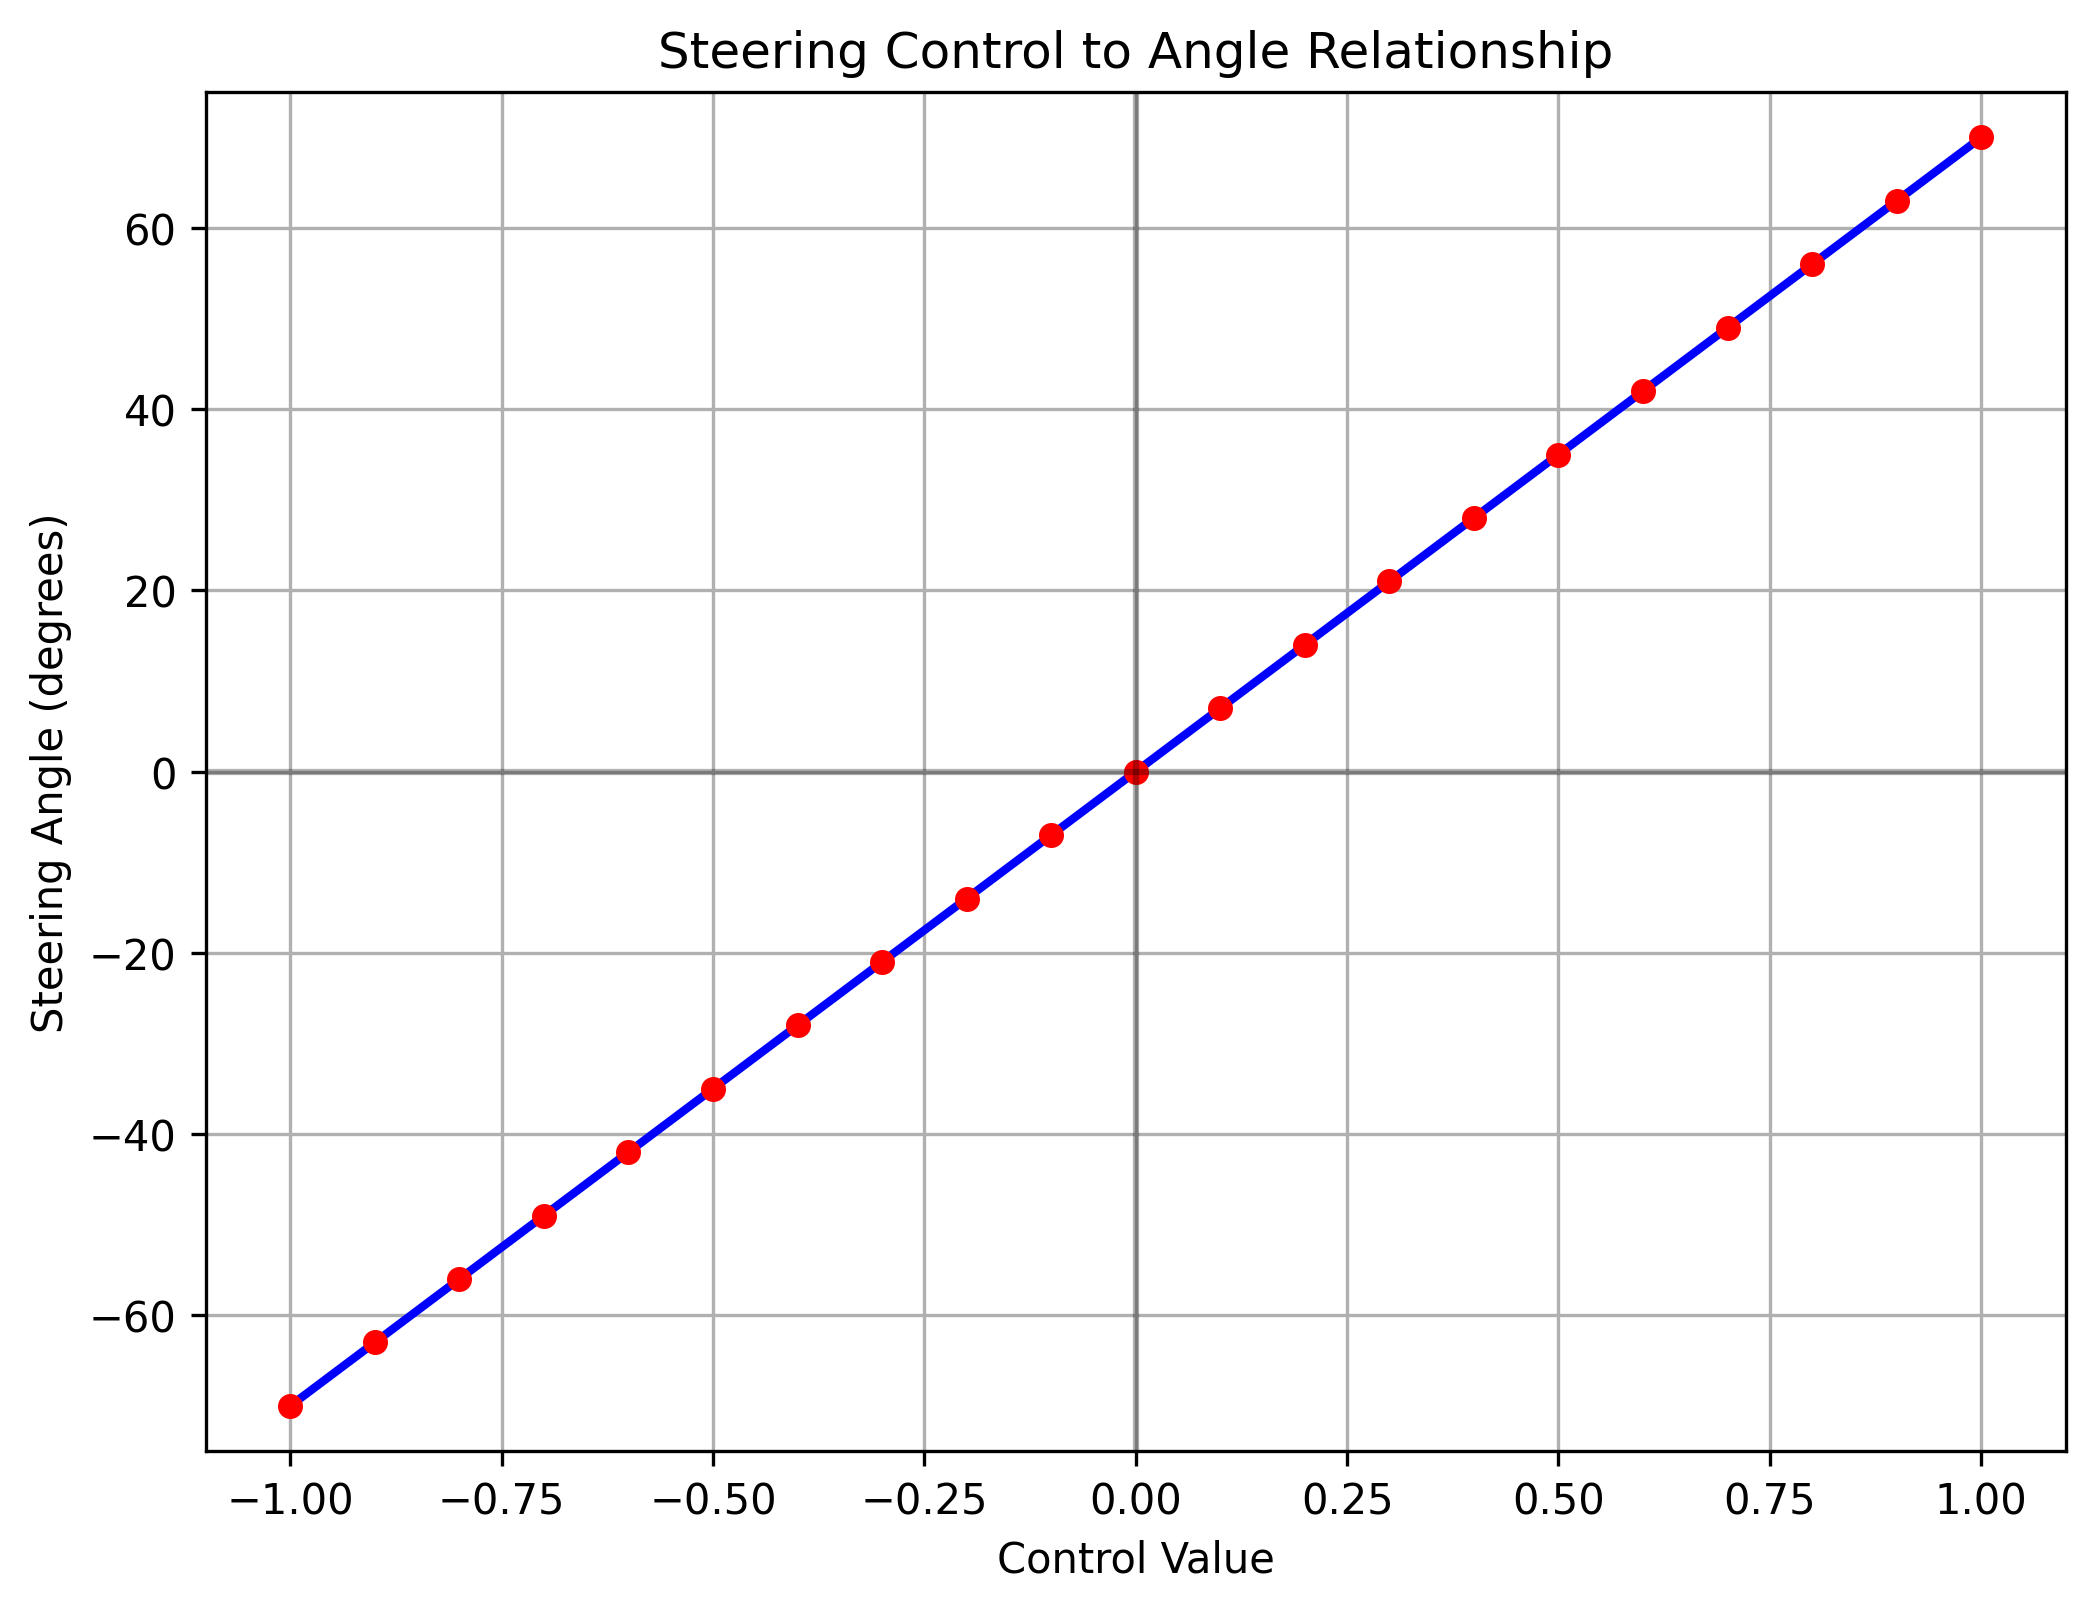
\includegraphics[width=0.8\textwidth]{Figures/Methods/steering_relationship.png}
    \caption{Linear relationship between steering control input and resulting steering angle. Control values range from -1.0 (maximum left turn) to 1.0 (maximum right turn), mapping linearly to steering angles from -70° to 70°.}
    \label{fig:steering_relationship}
\end{figure}

The linear relationship between control inputs and steering angles is demonstrated in Figure \ref{fig:steering_relationship}. The plot illustrates the direct proportional relationship, with control values of -1.0 and 1.0 corresponding precisely to the vehicle's maximum steering angles of -70° and 70° respectively. This linear mapping ensures predictable and intuitive vehicle control behavior throughout the entire steering range.

The video \url{https://youtu.be/cg6hhrpsc5g} shows experiments conducted in the CARLA simulator using a Tesla Model 3 vehicle. The experiments, documented in a Jupyter notebook\footnote{\url{https://github.com/dsikar/carla-driver-data/blob/main/scripts/04-steering-angle-study.ipynb}}, examine the vehicle's steering capabilities.

The vehicle demonstrates a maximum steering angle of 70 degrees in both directions, with steering control normalized between -1 (full left turn, -70 degrees) and 0 (neutral position) to +1 (full right turn, +70 degrees). The testing procedure follows a systematic sequence: starting from neutral (0°), turning gradually left to maximum (-70°), sweeping from full left to full right (+70°), and returning to center position, with each position maintained for 0.2 seconds.

The implemented visualization demonstrates a linear relationship between control values and actual steering angles, providing insights into the Tesla Model 3's steering behavior for understanding vehicle dynamics and control systems.

The steering angle logging process utilizes Python's logging module to record the Tesla Model 3's steering control values in CARLA simulation. The implementation creates a file handler that writes timestamped logs to \texttt{carla\_simulation.log}, recording steering values between -1 (full left) and 1 (full right) at 0.2-second intervals. The logging function \texttt{log\_steering\_control()} operates while the vehicle is under autopilot control, with a camera manager providing a back-right diagonal view for visual monitoring of the vehicle's behavior during data collection.

\subsection{Controlling Carla Weather}
The CARLA simulator's weather system is controlled through the \texttt{WeatherParameters} class, which manages sun position and atmospheric conditions. The sun's position is defined by two key parameters: altitude angle (range -90° to 90°, where -90° represents night, 0° horizon, and 90° directly overhead) and azimuth angle (0°/360° North, 90° East, 180° South, 270° West). Additional parameters include cloudiness, precipitation, precipitation deposits, and fog density, all ranging from 0 to 100. Preset weather configurations are implemented for typical daylight phases: morning (15° altitude, 90° azimuth), noon (90° altitude, 180° azimuth), afternoon (45° altitude, 270° azimuth), sunset (10° altitude, 270° azimuth), and night (-90° altitude, 270° azimuth).

\subsection{Determining waypoints for PID lane following}

\begin{align*}
\text{Waypoint} &= \{id, transform, road\_id, section\_id, lane\_id, s\} \\
transform &= \{location(x,y,z), rotation(pitch,yaw,roll)\} \\
lane\_properties &= \{lane\_width, lane\_type, lane\_change, left\_marking, right\_marking\} \\
junction\_data &= \{is\_junction, is\_intersection, junction\_id\}
\end{align*}

These properties enable waypoint-based navigation:
\begin{itemize}
\item $s$ measures distance along road segment
\item $lane\_id < 0$ for right lanes, $> 0$ for left lanes
\item $road\_id$ groups waypoints into road segments
\item $transform$ provides 3D pose for trajectory following
\item $lane\_change \in \{None, Left, Right, Both\}$ defines allowed transitions
\end{itemize}

\subsection{Maximum Distance Between Centroids}

The maximum distance between two points in an n-dimensional space depends on the constraints applied to the coordinates. For probability distributions, each coordinate must be non-negative, and the sum of all coordinates must equal 1. These constraints define a simplex in the n-dimensional space. For a vector $\mathbf{p} = (p_1, ..., p_n)$ in this space:

\begin{equation}
\sum_{i=1}^n p_i = 1 \quad \text{and} \quad p_i \geq 0 \quad \forall i
\end{equation}

The maximum Euclidean distance between two points in this simplex occurs between vertices. Each vertex has one coordinate equal to 1 and all others equal to 0. The Euclidean distance $d$ between two vertices $\mathbf{p}$ and $\mathbf{q}$ is:

\begin{equation}
d(\mathbf{p}, \mathbf{q}) = \sqrt{\sum_{i=1}^n (p_i - q_i)^2}
\end{equation}

For two vertices that differ in positions $j$ and $k$, we have $p_j = 1$, $q_j = 0$, $p_k = 0$, $q_k = 1$, and all other coordinates are 0. This gives:

\begin{equation}
d(\mathbf{p}, \mathbf{q}) = \sqrt{(1-0)^2 + (0-1)^2} = \sqrt{2}
\end{equation}

This maximum distance applies to neural networks with softmax outputs. A prediction for class $j$ produces a vector with maximum probability at position $j$. When the network assigns probability 1 to a class, the output is a vertex of the simplex. The distance between predictions of different classes reaches its maximum of $\sqrt{2}$ when the network assigns probability 1 to each class i.e. in the Softmax output array.

The maximum distance between two points in an n-dimensional space depends on the constraints applied to the coordinates. For probability distributions, each coordinate must be non-negative, and the sum of all coordinates must equal 1. These constraints define a simplex in the n-dimensional space. For a vector $\mathbf{p} = (p_1, ..., p_n)$ in this space:

\begin{equation}
\sum_{i=1}^n p_i = 1 \quad \text{and} \quad p_i \geq 0 \quad \forall i
\end{equation}

The maximum Euclidean distance between two points in this simplex occurs between vertices. Each vertex has one coordinate equal to 1 and all others equal to 0. The Euclidean distance $d$ between two vertices $\mathbf{p}$ and $\mathbf{q}$ is:

\begin{equation}
d(\mathbf{p}, \mathbf{q}) = \sqrt{\sum_{i=1}^n (p_i - q_i)^2}
\end{equation}

For two vertices that differ in positions $j$ and $k$, we have $p_j = 1$, $q_j = 0$, $p_k = 0$, $q_k = 1$, and all other coordinates are 0. This gives:

\begin{equation}
d(\mathbf{p}, \mathbf{q}) = \sqrt{(1-0)^2 + (0-1)^2} = \sqrt{2}
\end{equation}

This maximum distance applies to neural networks with softmax outputs. A prediction for class $j$ produces a vector with maximum probability at position $j$. When the network assigns probability 1 to a class, the output is a vertex of the simplex. The distance between predictions of different classes reaches its maximum of $\sqrt{2}$ when the network assigns probability 1 to each class.

The geometry of this space has properties that differ from standard Euclidean space. While we use Euclidean distance as a metric, the vertices of the probability simplex form an equilateral simplex where all pairwise distances are equal to $\sqrt{2}$. The angles between any two vertices are $arccos(-\frac{1}{n-1}) \approx 60°$ in degrees, not 90° as might be expected from intuition in Euclidean space. Alternative distance measures for probability distributions, such as the Kullback-Leibler divergence, can capture different aspects of the relationship between points:

\begin{equation}
D_{KL}(\mathbf{p}||\mathbf{q}) = \sum_{i=1}^n p_i \log\frac{p_i}{q_i}
\end{equation}

% The choice of distance metric affects the interpretation of the relationships between centroids in the softmax output space.

\subsection{Training dataset Town04}

We collected images and steering angles from a PID driving algorithm.

\begin{verbatim}
Dataset Summary:
--------------------------------------------------
Total images: 15840

Steering Angle Statistics:
count    15840.000000
mean         0.000534
std          0.018029
min         -0.077800
25%         -0.007500
50%         -0.000000
75%          0.001700
max          0.158000
Name: steering_angle, dtype: float64


Additional Statistics:
--------------------------------------------------
Absolute mean steering angle: 0.0100
Standard deviation: 0.0180
Maximum absolute steering angle: 0.1580
Percentage of straight driving (|angle| < 0.01): 58.0%    
\end{verbatim}

\begin{figure}
    \centering
    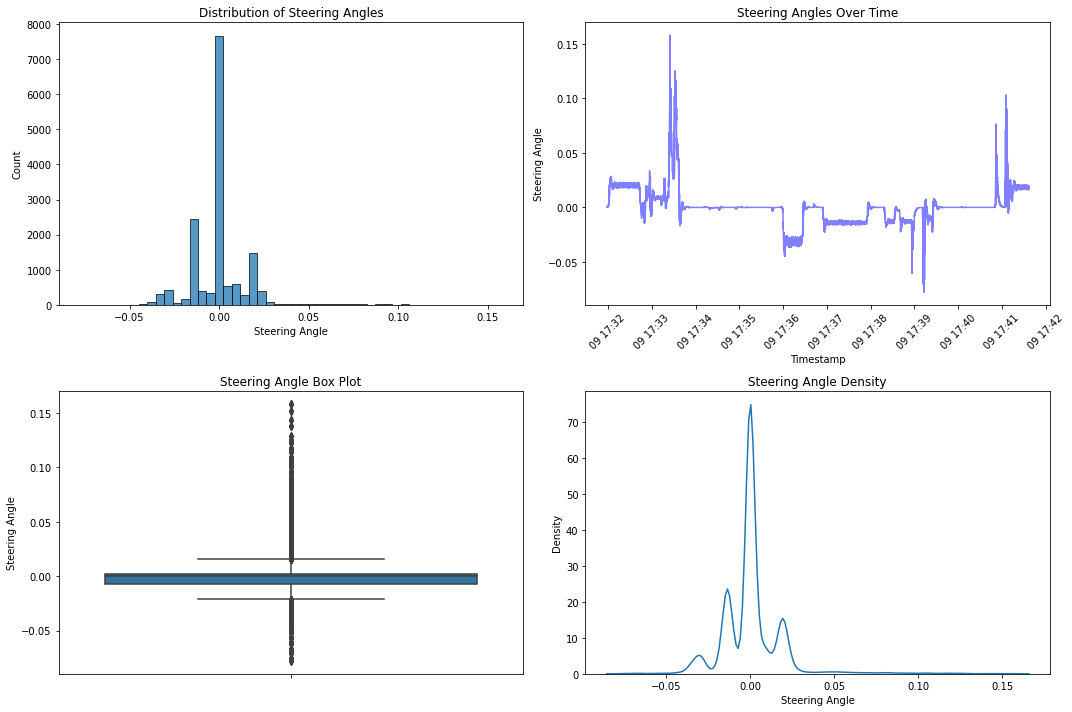
\includegraphics[width=0.99\linewidth]{Figures/Methods/Steering-Angle-Data-Town04-commit-04e147a.png}
    \caption{Caption}
    \label{fig:Steering-Angle-Data-Town04-commit-04e147a}
\end{figure}

\begin{figure}
    \centering
    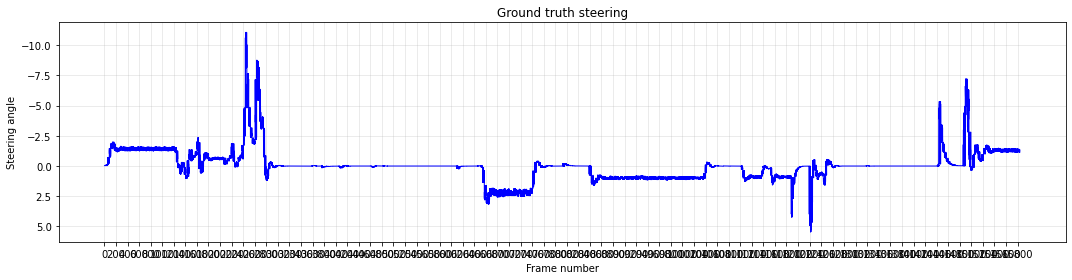
\includegraphics[width=0.99\linewidth]{Figures/Methods/Steering-Angle-2-Data-Town04-commit-ab3363b.png}
    \caption{Steering angle around figure of eight track}
    \label{fig:Steering-Angle-2-Data-Town04-commit-ab3363b.png}
\end{figure}

%% Image crop section

% ~/git/carla-driver-data/scripts/14-image-cropping-and-pre-processing.ipynb

\begin{figure}
    \centering
    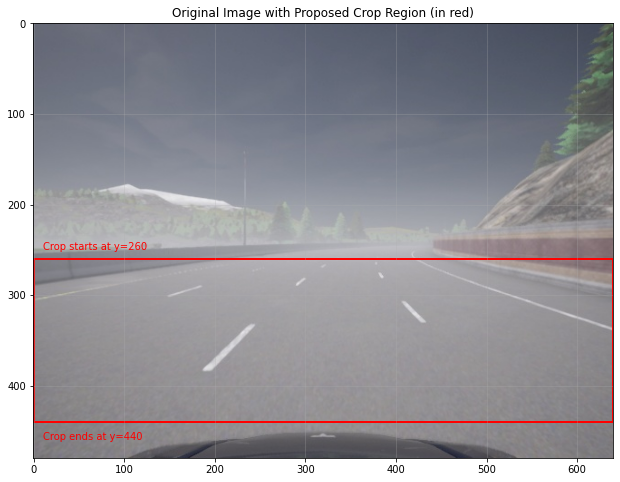
\includegraphics[width=0.99\linewidth]{Figures/Methods/Carla-Image-Crop-Area-Town04-2c3284c.png}
    \caption{Caption}
    \label{fig:Carla-Image-Crop-Area-Town04-2c3284c.png}
\end{figure}

%% Image crop section resized and moved to YUV space

\begin{figure}
    \centering
    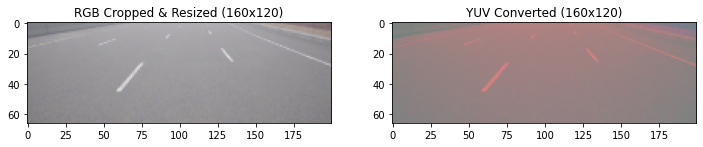
\includegraphics[width=0.99\linewidth]{Figures/Methods/Carla-Image-Crop-Resize-YUV-Town04-commit-2c3284c.png}
    \caption{Caption}
    \label{fig:Carla-Image-Crop-Resize-YUV-Town04-commit-2c3284c.png}
\end{figure}

\subsection{Town04 Figure of 8}
\subsection{Road ID selection}
\subsection{Camera placement}

\subsection{Camera Parameters}
In real-world self-driving systems, the camera parameters are carefully chosen to balance \textbf{field of view (FOV)}, \textbf{resolution}, \textbf{frame rate}, and \textbf{dynamic range} to ensure robust perception in various driving conditions. Below are realistic parameters for cameras used in autonomous vehicles, along with explanations for each.

\subsubsection{Field of View (FOV)}
\begin{itemize}
    \item \textbf{Typical FOV}: \textbf{60° to 120°}
    \begin{itemize}
        \item \textbf{Wide FOV (120°)}:
        \begin{itemize}
            \item Used for \textbf{short-range perception} (e.g., detecting pedestrians, obstacles, and lane markings close to the vehicle).
            \item Provides a broader view but introduces more distortion at the edges.
        \end{itemize}
        \item \textbf{Narrow FOV (60°)}:
        \begin{itemize}
            \item Used for \textbf{long-range perception} (e.g., detecting traffic signs, vehicles, and road conditions far ahead).
            \item Provides a more focused view with less distortion.
        \end{itemize}
    \end{itemize}
    \item \textbf{Why It Matters}:
    \begin{itemize}
        \item A wider FOV is better for urban driving, where the vehicle needs to detect objects in close proximity.
        \item A narrower FOV is better for highway driving, where the focus is on distant objects.
    \end{itemize}
\end{itemize}

\subsubsection{Resolution}
\begin{itemize}
    \item \textbf{Typical Resolution}: \textbf{1280x720 (HD)} to \textbf{1920x1080 (Full HD)}
    \begin{itemize}
        \item \textbf{1280x720 (HD)}:
        \begin{itemize}
            \item Suitable for \textbf{basic object detection} and \textbf{lane tracking}.
            \item Lower computational requirements.
        \end{itemize}
        \item \textbf{1920x1080 (Full HD)}:
        \begin{itemize}
            \item Provides more detail for \textbf{fine-grained tasks} like traffic sign recognition, pedestrian detection, and lane marking segmentation.
            \item Higher computational requirements.
        \end{itemize}
    \end{itemize}
    \item \textbf{Why It Matters}:
    \begin{itemize}
        \item Higher resolution improves the accuracy of object detection and classification but increases the computational load.
    \end{itemize}
\end{itemize}

\subsubsection{Frame Rate}
\begin{itemize}
    \item \textbf{Typical Frame Rate}: \textbf{20 FPS to 60 FPS}
    \begin{itemize}
        \item \textbf{20 FPS}:
        \begin{itemize}
            \item Suitable for \textbf{low-speed driving} or \textbf{static environments}.
        \end{itemize}
        \item \textbf{30 FPS}:
        \begin{itemize}
            \item Commonly used in real-world systems for a balance between performance and computational cost.
        \end{itemize}
        \item \textbf{60 FPS}:
        \begin{itemize}
            \item Used for \textbf{high-speed driving} or \textbf{dynamic environments} where rapid changes need to be captured.
        \end{itemize}
    \end{itemize}
    \item \textbf{Why It Matters}:
    \begin{itemize}
        \item Higher frame rates improve the system's ability to track fast-moving objects but require more processing power.
    \end{itemize}
\end{itemize}

\subsubsection{Dynamic Range}
\begin{itemize}
    \item \textbf{Typical Dynamic Range}: \textbf{100 dB to 120 dB}
    \begin{itemize}
        \item \textbf{High Dynamic Range (HDR)}:
        \begin{itemize}
            \item Ensures the camera can capture details in both \textbf{bright} (e.g., sunlight) and \textbf{dark} (e.g., shadows) areas of the scene.
            \item Critical for handling challenging lighting conditions (e.g., driving into the sun or through tunnels).
        \end{itemize}
    \end{itemize}
    \item \textbf{Why It Matters}:
    \begin{itemize}
        \item Without HDR, the camera may overexpose or underexpose parts of the image, leading to missed detections.
    \end{itemize}
\end{itemize}

\subsubsection{Mounting Position}
\begin{itemize}
    \item \textbf{Typical Height}: \textbf{1.5 to 2.5 meters above the ground}
    \begin{itemize}
        \item Mounted on the \textbf{roof} or \textbf{windshield} of the vehicle.
        \item Provides a clear view of the road ahead while minimizing obstructions.
    \end{itemize}
    \item \textbf{Typical Pitch}: \textbf{-10° to -20°}
    \begin{itemize}
        \item Tilted slightly downward to focus on the road and nearby objects.
    \end{itemize}
    \item \textbf{Why It Matters}:
    \begin{itemize}
        \item The mounting position and angle determine the camera's coverage and ability to detect objects at different distances.
    \end{itemize}
\end{itemize}

\subsubsection{Number of Cameras}
\begin{itemize}
    \item \textbf{Typical Setup}: \textbf{6 to 12 cameras}
    \begin{itemize}
        \item \textbf{Front-facing cameras}: 1–3 cameras with varying FOVs (e.g., narrow, medium, wide).
        \item \textbf{Side-facing cameras}: 2–4 cameras for blind spot detection and lane changes.
        \item \textbf{Rear-facing cameras}: 1–2 cameras for parking and rear obstacle detection.
        \item \textbf{Surround-view cameras}: 4–6 cameras for 360° perception.
    \end{itemize}
    \item \textbf{Why It Matters}:
    \begin{itemize}
        \item Multiple cameras provide redundancy and coverage of the entire environment around the vehicle.
    \end{itemize}
\end{itemize}

\subsubsection{Realistic Camera Parameters for Self-Driving Systems}
Below is an example of realistic camera parameters for a front-facing camera in a self-driving system:

\begin{table}[h!]
    \centering
    \begin{tabular}{|l|l|}
        \hline
        \textbf{Parameter} & \textbf{Value} \\
        \hline
        Resolution & 1920x1080 (Full HD) \\
        Frame Rate & 30 FPS \\
        Field of View & 90° (medium FOV) \\
        Dynamic Range & 120 dB (HDR) \\
        Mounting Height & 1.8 meters above the ground \\
        Mounting Pitch & -15° (tilted downward) \\
        \hline
    \end{tabular}
    \caption{Realistic Camera Parameters for a Front-Facing Camera}
    \label{tab:camera_params}
\end{table}

\subsection{Camera Placement}

% Image generated by scripts/23-camera-placement-study.ipynb/23-camera-placement-study.ipynb, function side_view_left_close(world, base_transform),


Figure \ref{fig:/tesla-model-3-camera-location} shows the approximate location of the camera: 1 distance unit along the x axis and 1.8 units along the z axis from the centre of the Tesla model 3 vehicle. Figure \ref{fig:/tesla-model-3-camera-image} shows the captured image with the parameters 

\begin{figure}[h]
    \centering
    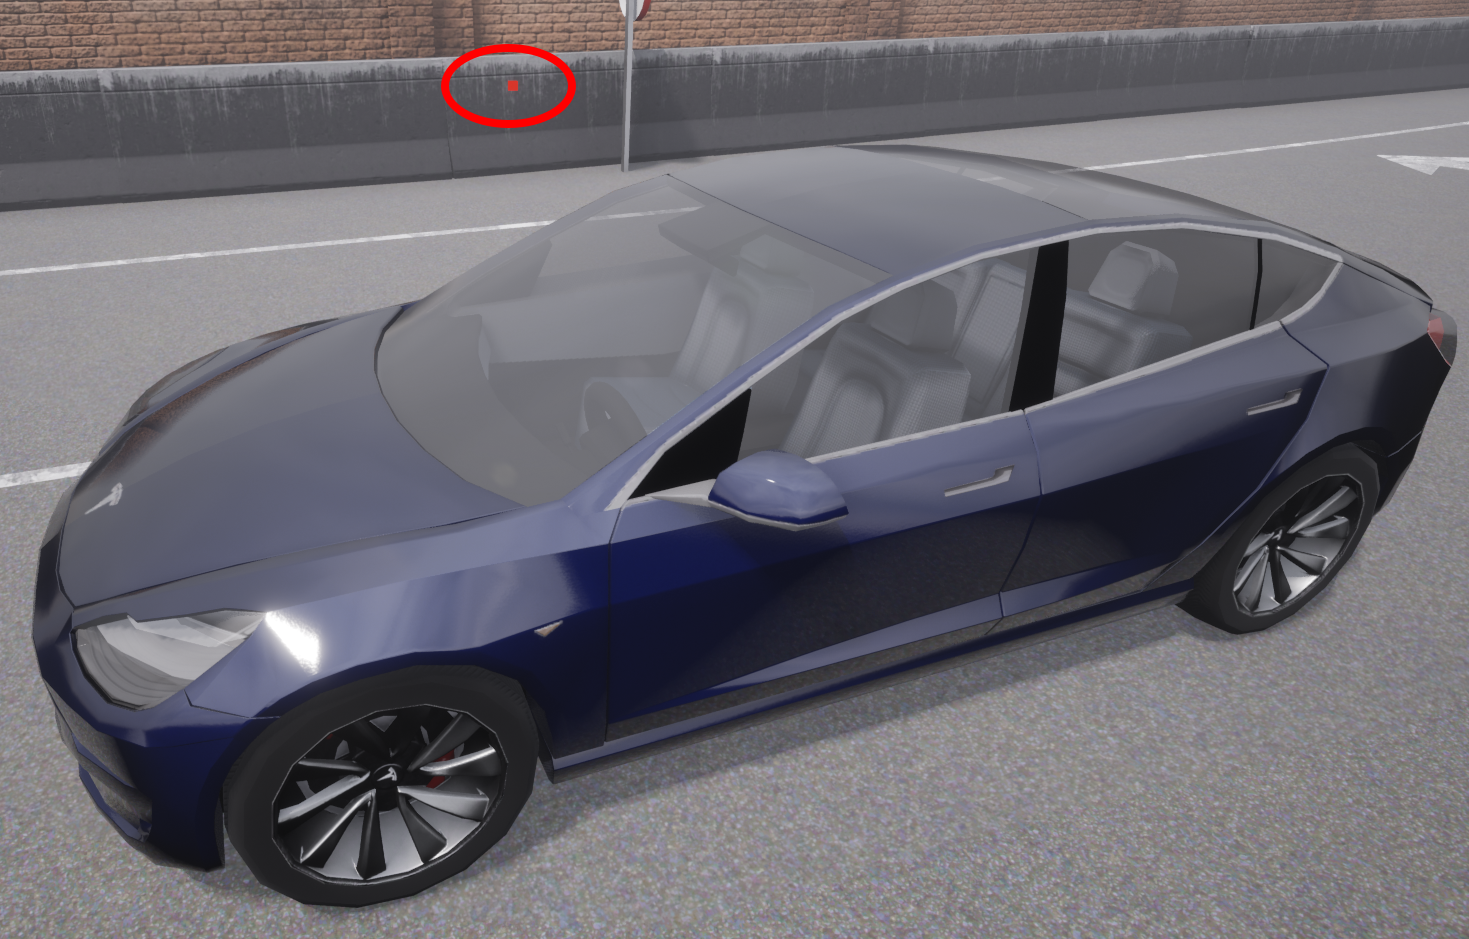
\includegraphics[width=0.75\textwidth]{Figures/Methods/tesla-model-3-camera-location.png}
    \caption{CARLA Tesla model 3 on Figure of 8 Road. Red Ellipsis is approximate location of camera.}
    \label{fig:/tesla-model-3-camera-location}
\end{figure}

\begin{figure}[h]
    \centering
    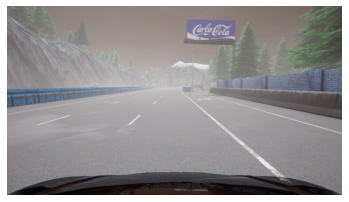
\includegraphics[width=0.75\textwidth]{Figures/Methods/tesla-model-3-camera-image.png}
    \caption{Example camera image capture showing the end of the hood at the bottom.}
    \label{fig:/tesla-model-3-camera-image}
\end{figure}

The camera in the CarlaRecorder is positioned at coordinates (1.5, 0.0, 1.8) relative to the vehicle's center. This places the camera 1.5 meters forward along the vehicle's x-axis, directly centered on the y-axis (0.0), and 1.8 meters up from the vehicle's base on the z-axis. The camera uses a rotation of (pitch=-5.0, yaw=0.0, roll=0.0), which points the camera slightly downward at a 5-degree angle while maintaining forward alignment with the vehicle's direction. This camera configuration provides a view of the road ahead from a position that approximates a dashboard or windshield-mounted camera in a real vehicle. The camera captures images at a resolution defined by image\_width and image\_height parameters (default 640×480 pixels) and uses a field of view parameter (default 90 degrees) to determine the camera's viewing angle.



\begin{verbatim}
Number of waypoints retrieved: 3063
Vehicle spawned at Location(x=160.342804, y=-368.140472, z=0.100000)
Camera attached to vehicle at Location(x=1.000000, y=0.000000, z=1.400000)
Image size verified successfully.
Camera parameters FOV:90, Image Size:(1920, 1080)
Camera position: Location(x=161.342758, y=-368.131714, z=1.403298)
Camera rotation: Rotation(pitch=-4.999999, yaw=0.501399, roll=0.000000)
\end{verbatim}

%%%%%%%%%%%%%%%%
% CAMERA STUDY %
%%%%%%%%%%%%%%%%

\begin{figure}[h]
    \centering
    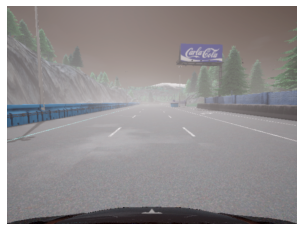
\includegraphics[width=0.75\textwidth]{Figures/Methods/640x480_90_1.4_1.4_lane_id_minus_2.png}
    \caption{Example camera image capture showing the end of the hood at the bottom, on lane id -2.}
    \label{fig:/640x480_90_1.4_1.4_lane_id_minus_2}
\end{figure}

Code to generate Figure \ref{fig:/640x480_90_1.4_1.4_lane_id_minus_2}:

\begin{verbatim}
scripts/02-camera-study.ipynb

camera_config = {
    "width": 640,
    "height": 480,
    "fov": 90,
    "position": carla.Location(x=1.4, y=0.0, z=1.4),
    "rotation": carla.Rotation(pitch=-5.0, yaw=0.0, roll=0.0)
}
test_vehicle_and_camera(world, vehicle, camera_config)

\end{verbatim}

%%%%%%%%%%%%%%%%%%%%%%%%%%%
% LANE SEGMENTATION STUDY %
%%%%%%%%%%%%%%%%%%%%%%%%%%%

\begin{figure}[h]
    \centering
    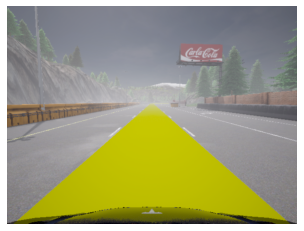
\includegraphics[width=0.75\textwidth]{Figures/Methods/640x480_90_1.4_1.4_lane_id_minus_2_segmented.png}
    \caption{Example camera image capture showing the end of the hood at the bottom, on lane id -2.}
    \label{fig:/640x480_90_1.4_1.4_lane_id_minus_2_segmented}
\end{figure}

Code to generate Figure \ref{fig:/640x480_90_1.4_1.4_lane_id_minus_2_segmented}:

\begin{verbatim}
scripts/03-lane-segmentation.ipynb

draw_permanent_waypoint_lines(world, waypoints_2, color=carla.Color(35, 35, 0), thickness=1.5, life_time=0)
(...)
# Example usage
camera_config = {
    "width": 640,
    "height": 480,
    "fov": 90,
    "position": carla.Location(x=1.4, y=0.0, z=1.4),
    "rotation": carla.Rotation(pitch=-5.0, yaw=0.0, roll=0.0)
}
test_vehicle_and_camera(world, vehicle, camera_config)
\end{verbatim}

%%%%%%%%%%%%%%%%%%%%%%%%%
% WITH FIDUCIAL MARKERS %
%%%%%%%%%%%%%%%%%%%%%%%%%

\begin{figure}[h]
    \centering
    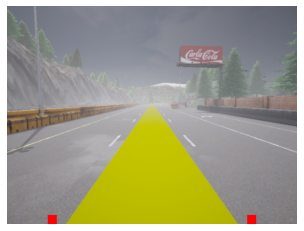
\includegraphics[width=0.75\textwidth]{Figures/Methods/640x480_90_1.4_1.4_lane_id_minus_2_segmented_with_fiducials.png}
    \caption{Example camera image capture showing the end of the hood at the bottom, on lane id -2.}
    \label{fig:/640x480_90_1.4_1.4_lane_id_minus_2_segmented}
\end{figure}

Code to generate Figure \ref{fig:/640x480_90_1.4_1.4_lane_id_minus_2_segmented_with_fiducials}:

\begin{verbatim}
scripts/04-fiducial-markers.ipynb

draw_permanent_waypoint_lines(world, waypoints_2, color=carla.Color(35, 35, 0), thickness=1.5, life_time=0)
(...)
# Example usage
camera_config = {
    "width": 640,
    "height": 480,
    "fov": 90,
    "position": carla.Location(x=1.4, y=0.0, z=1.4),
    "rotation": carla.Rotation(pitch=-5.0, yaw=0.0, roll=0.0)
}
test_vehicle_and_camera_with_fiducial_markers(world, vehicle, camera_config)
\end{verbatim}

\subsection{Generating a training dataset with lane segmentation}

We generate two datasets, one with lane segmentation and another with lane segmentation and fiducial markers on either side of the segmented lane.

Figure \ref{steering_angle_distribution_carla_dataset_640x480_01} shows the distribution of steering angles for dataset 01 (segmentation only). The statistics are identical for both 01 and 02 datasets:

\begin{verbatim}
Mean: 0.0001
Standard Deviation: 0.0162
Variance: 0.0003
Minimum: -0.0811
Maximum: 0.1265
\end{verbatim}

\begin{figure}[h]
    \centering
    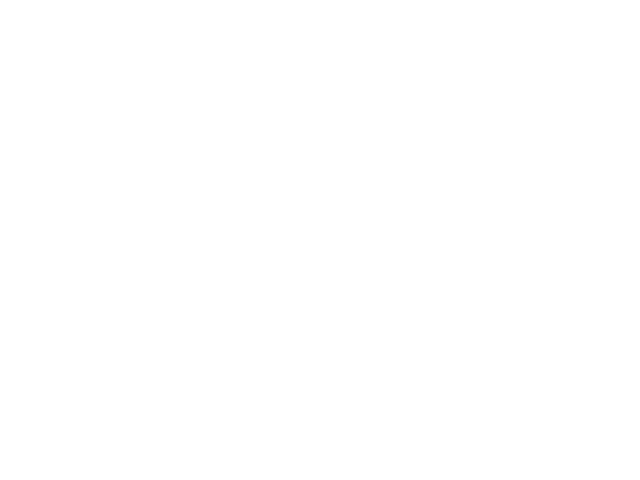
\includegraphics[width=0.75\textwidth]{Figures/Methods/steering_angle_distribution_carla_dataset_640x480_01.png}
    \caption{Distribution of steering angles for dataset 01 (segmentation only).}
    \label{fig:/steering_angle_distribution_carla_dataset_640x480_01}
\end{figure}

\textbf{Bin Statistics for Steering Angle Histogram}

Note, mean, std, etc, are identical for 01 and 02.

Given a dataset of steering angles extracted from filenames in the directory \texttt{carla\_dataset\_640x480\_01}, we compute the statistics for a histogram with 15 bins. The steering angles range from a minimum of $-0.0811$ to a maximum of $0.1265$. Below, we describe how the bin widths and edges are determined, including the relevant equations.

\textbf{Data Range}:
The range of the steering angles is calculated as the difference between the maximum and minimum values:
\begin{equation}
\text{Range} = \max(\text{angles}) - \min(\text{angles})
\end{equation}
Substituting the given values:
\begin{equation}
\text{Range} = 0.1265 - (-0.0811) = 0.1265 + 0.0811 = 0.2076
\end{equation}
Thus, the range of the steering angles is $0.2076$.

\textbf{Bin Width}: 
The histogram is divided into 15 equal-width bins. The bin width is computed by dividing the range by the number of bins:
\begin{equation}
\text{Bin Width} = \frac{\text{Range}}{\text{Number of Bins}}
\end{equation}
With 15 bins:
\begin{equation}
\text{Bin Width} = \frac{0.2076}{15} \approx 0.01384
\end{equation}
Each bin has a width of approximately $0.01384$.

\textbf{Bin Edges}: 
The histogram consists of 15 bins, defined by 16 bin edges, starting from the minimum value and incrementing by the bin width. The bin edges are given by:
\begin{equation}
\text{Edge}_i = \min(\text{angles}) + i \cdot \text{Bin Width}, \quad i = 0, 1, \ldots, 15
\end{equation}
Substituting the minimum value ($-0.0811$) and bin width ($0.01384$):
\begin{equation}
\text{Edge}_i = -0.0811 + i \cdot 0.01384
\end{equation}
The bin edges are approximately:
\[
[-0.0811, -0.0673, -0.0534, -0.0396, -0.0257, -0.0119, 0.0020, 0.0158, 0.0297, 0.0435, 0.0574, 0.0712, 0.0851, 0.0989, 0.1127, 0.1265]
\]
Each bin spans an interval such as $[-0.0811, -0.0673)$, $[-0.0673, -0.0534)$, and so forth, with the final bin being $[0.1127, 0.1265]$.

\textbf:{Summary}
The histogram of steering angles is constructed with 15 equal-width bins, where:
\begin{itemize}
    \item The data range is $0.2076$, calculated as $0.1265 - (-0.0811)$.
    \item The bin width is approximately $0.01384$, derived from $\frac{0.2076}{15}$.
    \item The bin edges are computed as $-0.0811 + i \cdot 0.01384$ for $i = 0$ to $15$.
\end{itemize}
These bins are used by Matplotlib's \texttt{plt.hist} function to visualize the distribution of steering angles, with each bin representing the frequency of angles within its interval.

\subsection{Generating a training dataset}

The vehicle is placed on the first waypoint of the figure of eight track. The word the complete track. The simulation is set to 

% Questions to answer:
The CarlaRecorder operates in synchronous mode, which is explicitly enabled through the enable\_synchronous\_mode() method when the recorder starts. In this mode, the simulation time advances in discrete, fixed steps defined by the fixed\_delta\_seconds parameter (defaulted to 0.05 seconds, or 20 frames per second). Unlike asynchronous mode where the simulation runs continuously in real-time, synchronous mode gives precise control over simulation timing by requiring explicit "tick" commands to advance to the next frame. This is crucial for ensuring consistent and reliable data recording, as it guarantees that each camera capture corresponds exactly to the vehicle state at that specific simulation step. During the driving sequence, the recorder advances time by calling self.world.tick() after processing each control input, ensuring that sensor data (images) and vehicle controls remain perfectly synchronized. This deterministic approach prevents timing-related issues that could arise in asynchronous mode, where variable processing times might lead to inconsistent data collection intervals.

%(carla-env) daniel@simbox ~/git/carla-driver-data/scripts (main)$ git commit -%m "Gathering data"
%[main 9968488]

\begin{verbatim}
Simulation Log
Start Time: 2025-03-14 09:30:00
End Time: 2025-03-14 09:47:16
Total Images Recorded: 25938
Camera Position: x=1.5, y=0.0, z=1.8
Camera Rotation: pitch=-5.0, yaw=0.0, roll=0.0
Camera Parameters: resolution=640x480, fov=90    
\end{verbatim}

% Synchronous mode

duration of the recording:

Start time: 2025-03-14 09:30:00
End time: 2025-03-14 09:47:16
Duration: 17 minutes and 16 seconds = 1,036 seconds

Since the simulation runs at 20 frames per second in synchronous mode, and assuming one image is captured per frame, the expected number of images would be:
Expected images = 1,036 seconds × 20 frames/second = 20,720 images
The log reports 25,938 images recorded, which is 5,218 more than expected based on a strict 20 FPS capture rate.
This difference could be explained by several factors:
The simulation might not maintain exactly 20 FPS throughout the entire recording
The recording process might capture multiple images in some frames
There could be timing differences between simulation steps and image capturing
The camera might be set to capture at a higher frequency than the simulation tick rate

The reported number is about 25\% higher than calculated, which suggests some inconsistency in the recording process. If an exact match between simulation steps and recorded images is critical, further investigation into the image capture implementation would be warranted.

%https://carla.readthedocs.io/en/0.9.13/adv_synchrony_timestep/
%% git add wip/carla_figure8_selfdrive_recorder.py 

\subsection{Training Data Analysis}

%% TODO, once network is training, need stats on steering angles
% home/daniel/.pyenv/versions/3.6.9/envs/carla-env/bin/python /home/daniel/git/carla-driver-data/scripts/wip/02-steering-angle-stats.py
% Number of images: 25939
% Mean steering angle: -0.0019
% Max steering angle: 0.0851
% Min steering angle: -0.0419
% Standard deviation: 0.0148

% (carla-env) daniel@simbox ~/git/carla-driver-data/scripts/wip (main)$ git add 02-steering-angle-stats.py 
% (carla-env) daniel@simbox ~/git/carla-driver-data/scripts/wip (main)$ git commit -m "Steering angle stats"
% [main 9e866f8] Steering angle stats

\begin{figure}[h]
    \centering
    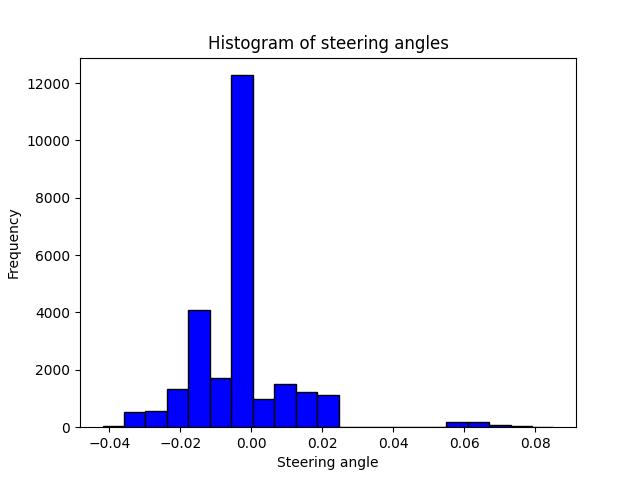
\includegraphics[width=0.55\textwidth]{Figures/Methods/steering_angle_histogram.png}
    \caption{21-bin histogram of steering angles Tesla model 3 on Figure of 8 Road.}
    \label{fig:/steering_angle_histogram}
\end{figure}

\subsection{Training the network}


% ~/dev/claude-dr/transformer-regressor/reports/analyze_steering_predictions.py 
% from run 119

\begin{figure}[h]
    \centering
    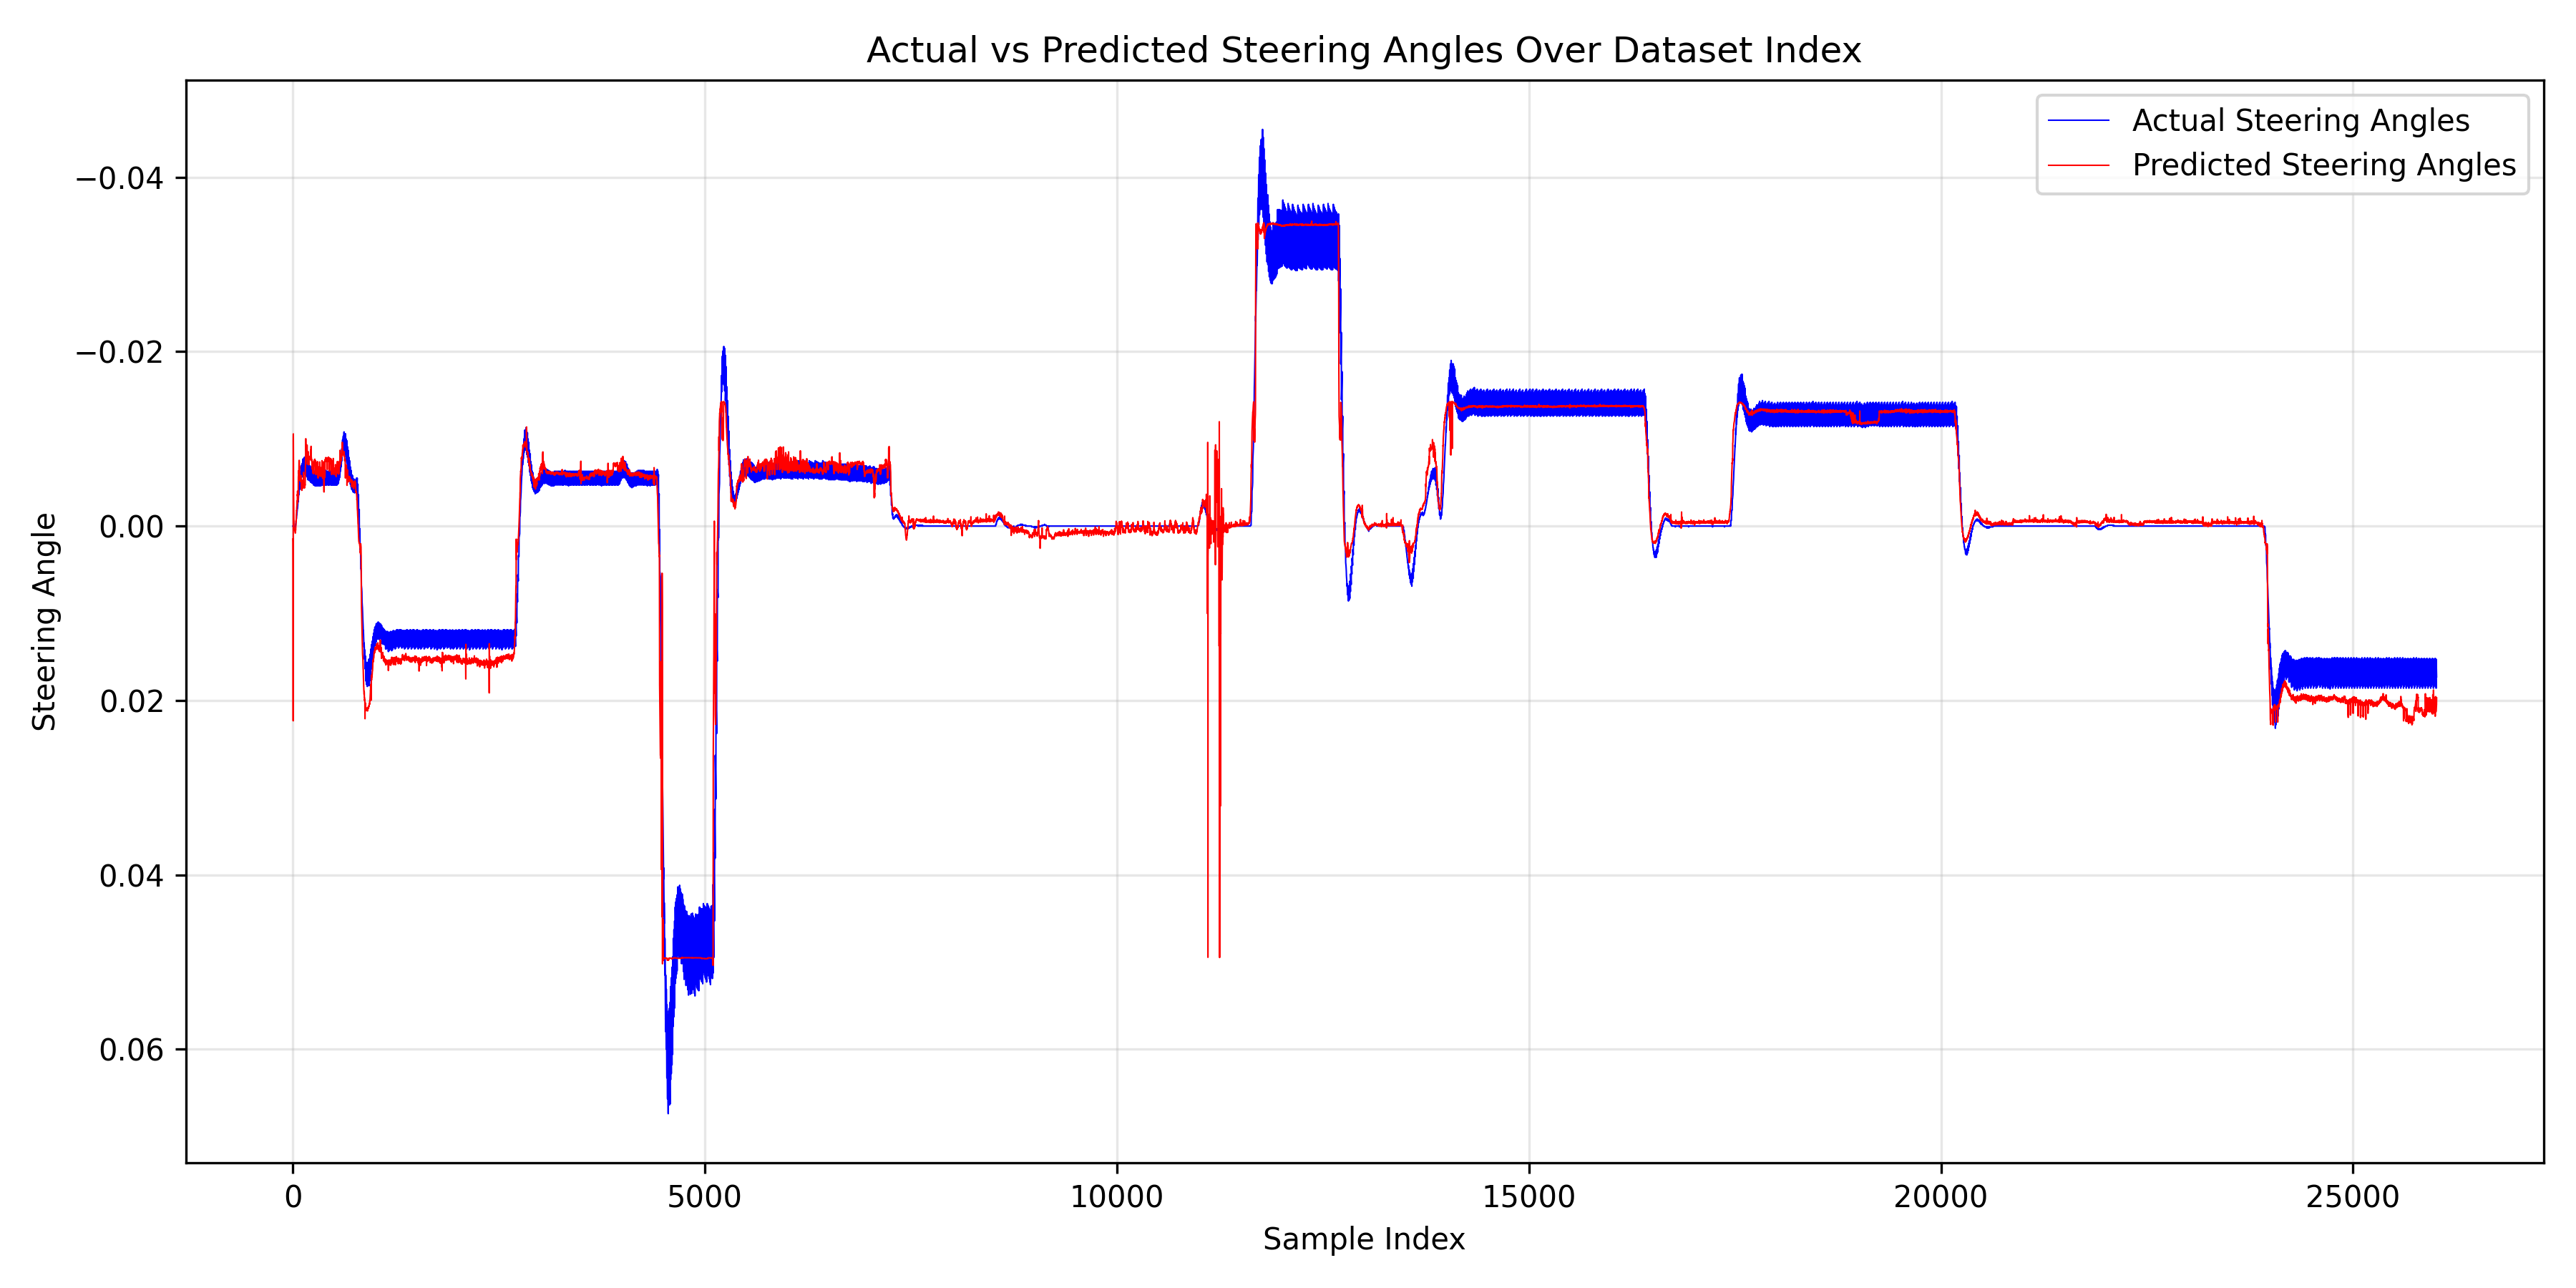
\includegraphics[width=0.99\textwidth]{Figures/Methods/predictions_vs_labels_vit.png}
    \caption{Predictions vs ground truth for ViT network, Town04}
    \label{fig:/predictions_vs_labels_vit}
\end{figure}

\begin{verbatim}

Steering Angle Statistics:
- Minimum: -0.045500
- Maximum: 0.067400
- Mean: -0.001549
- Median: 0.000000
- Standard Deviation: 0.013331
- Mean Absolute Value: 0.008690

Turn Direction Distribution:
- Left turns (< -0.001): 11465 (44.1%)
- Right turns (> 0.001): 5185 (19.9%)
- Neutral (straight): 9368 (36.0%)
- Total samples: 26018

\end{verbatim}

\begin{figure}[h]
    \centering
    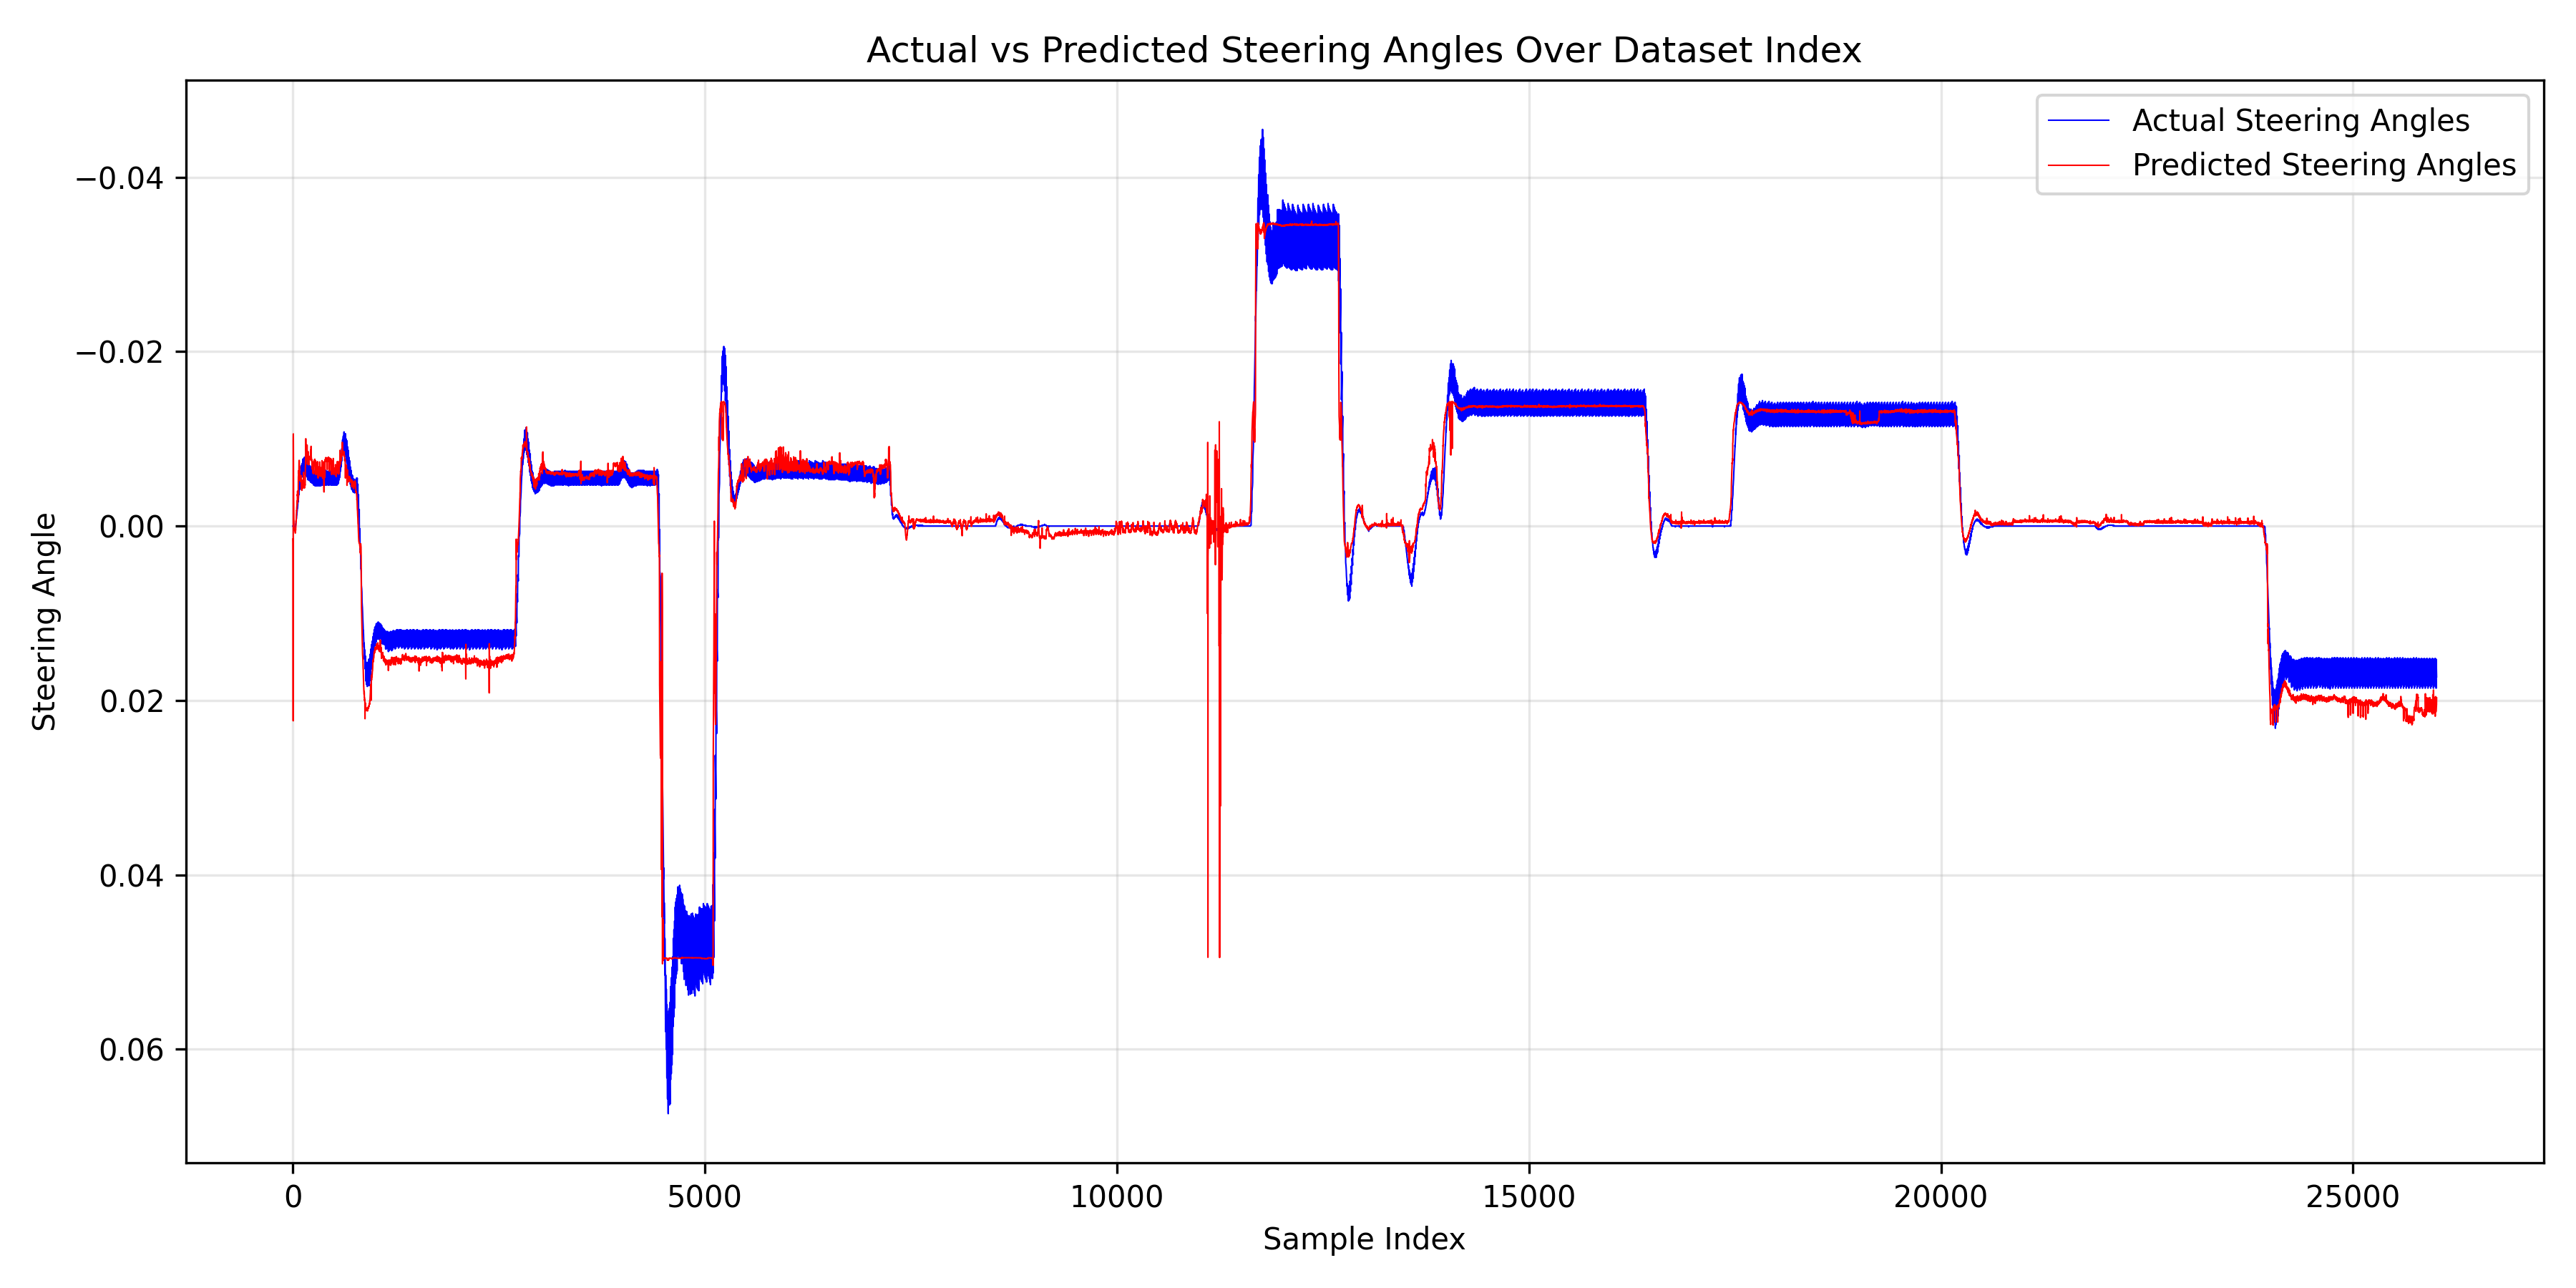
\includegraphics[width=0.99\textwidth]{Figures/Methods/predictions_vs_labels_vit.png}
    \caption{Predictions vs ground truth for ViT network, Town04}
    \label{fig:/predictions_vs_labels_vit}
\end{figure}

% TOWN04 Steering data

% (carla-env) daniel@simbox ~/git/carla-driver-data/reports (main)$ git commit -m "Added steering analytics"
% [main 2947160] Added steering analytics
%  1 file changed, 163 insertions(+)
%  create mode 100644 reports/laneid_1_analytics.py
\begin{figure}[h]
    \centering
    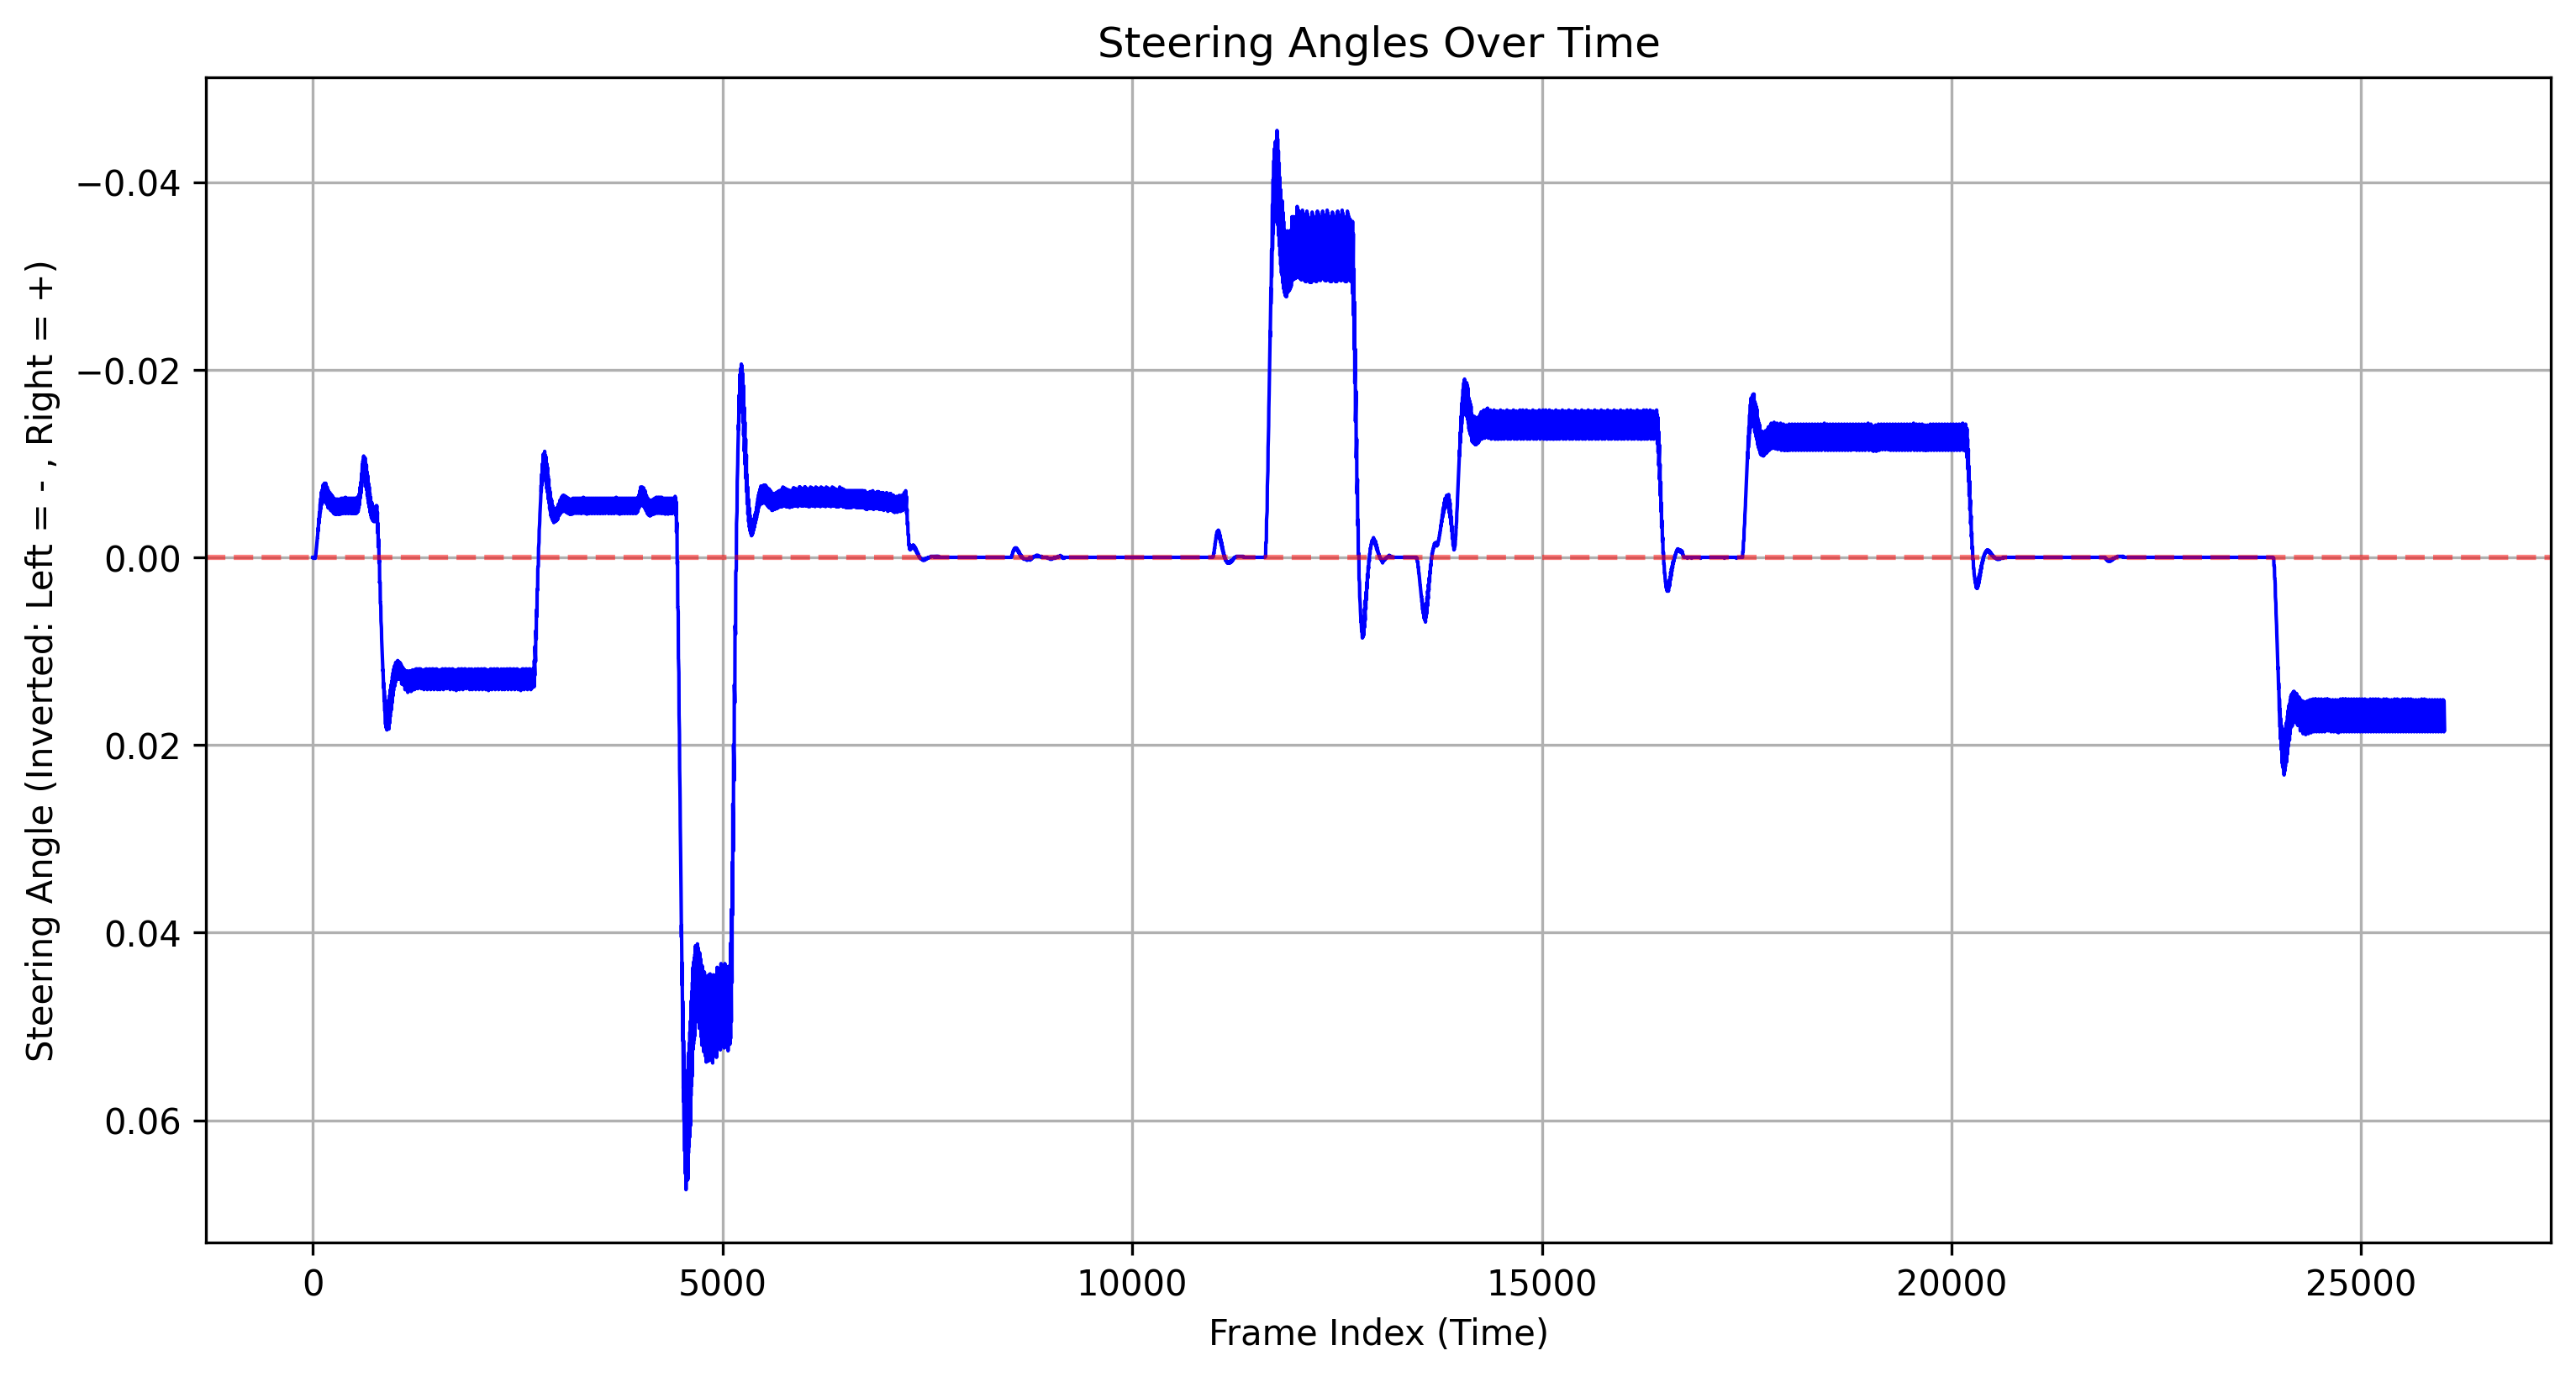
\includegraphics[width=0.99\textwidth]{Figures/Methods/steering_angles_town04.png}
    \caption{Ground truth steering around the entire figure 8 circuit (26k predictions, Town04}
    \label{fig:/steering_angles_town04}
\end{figure}

\begin{figure}[h]
    \centering
    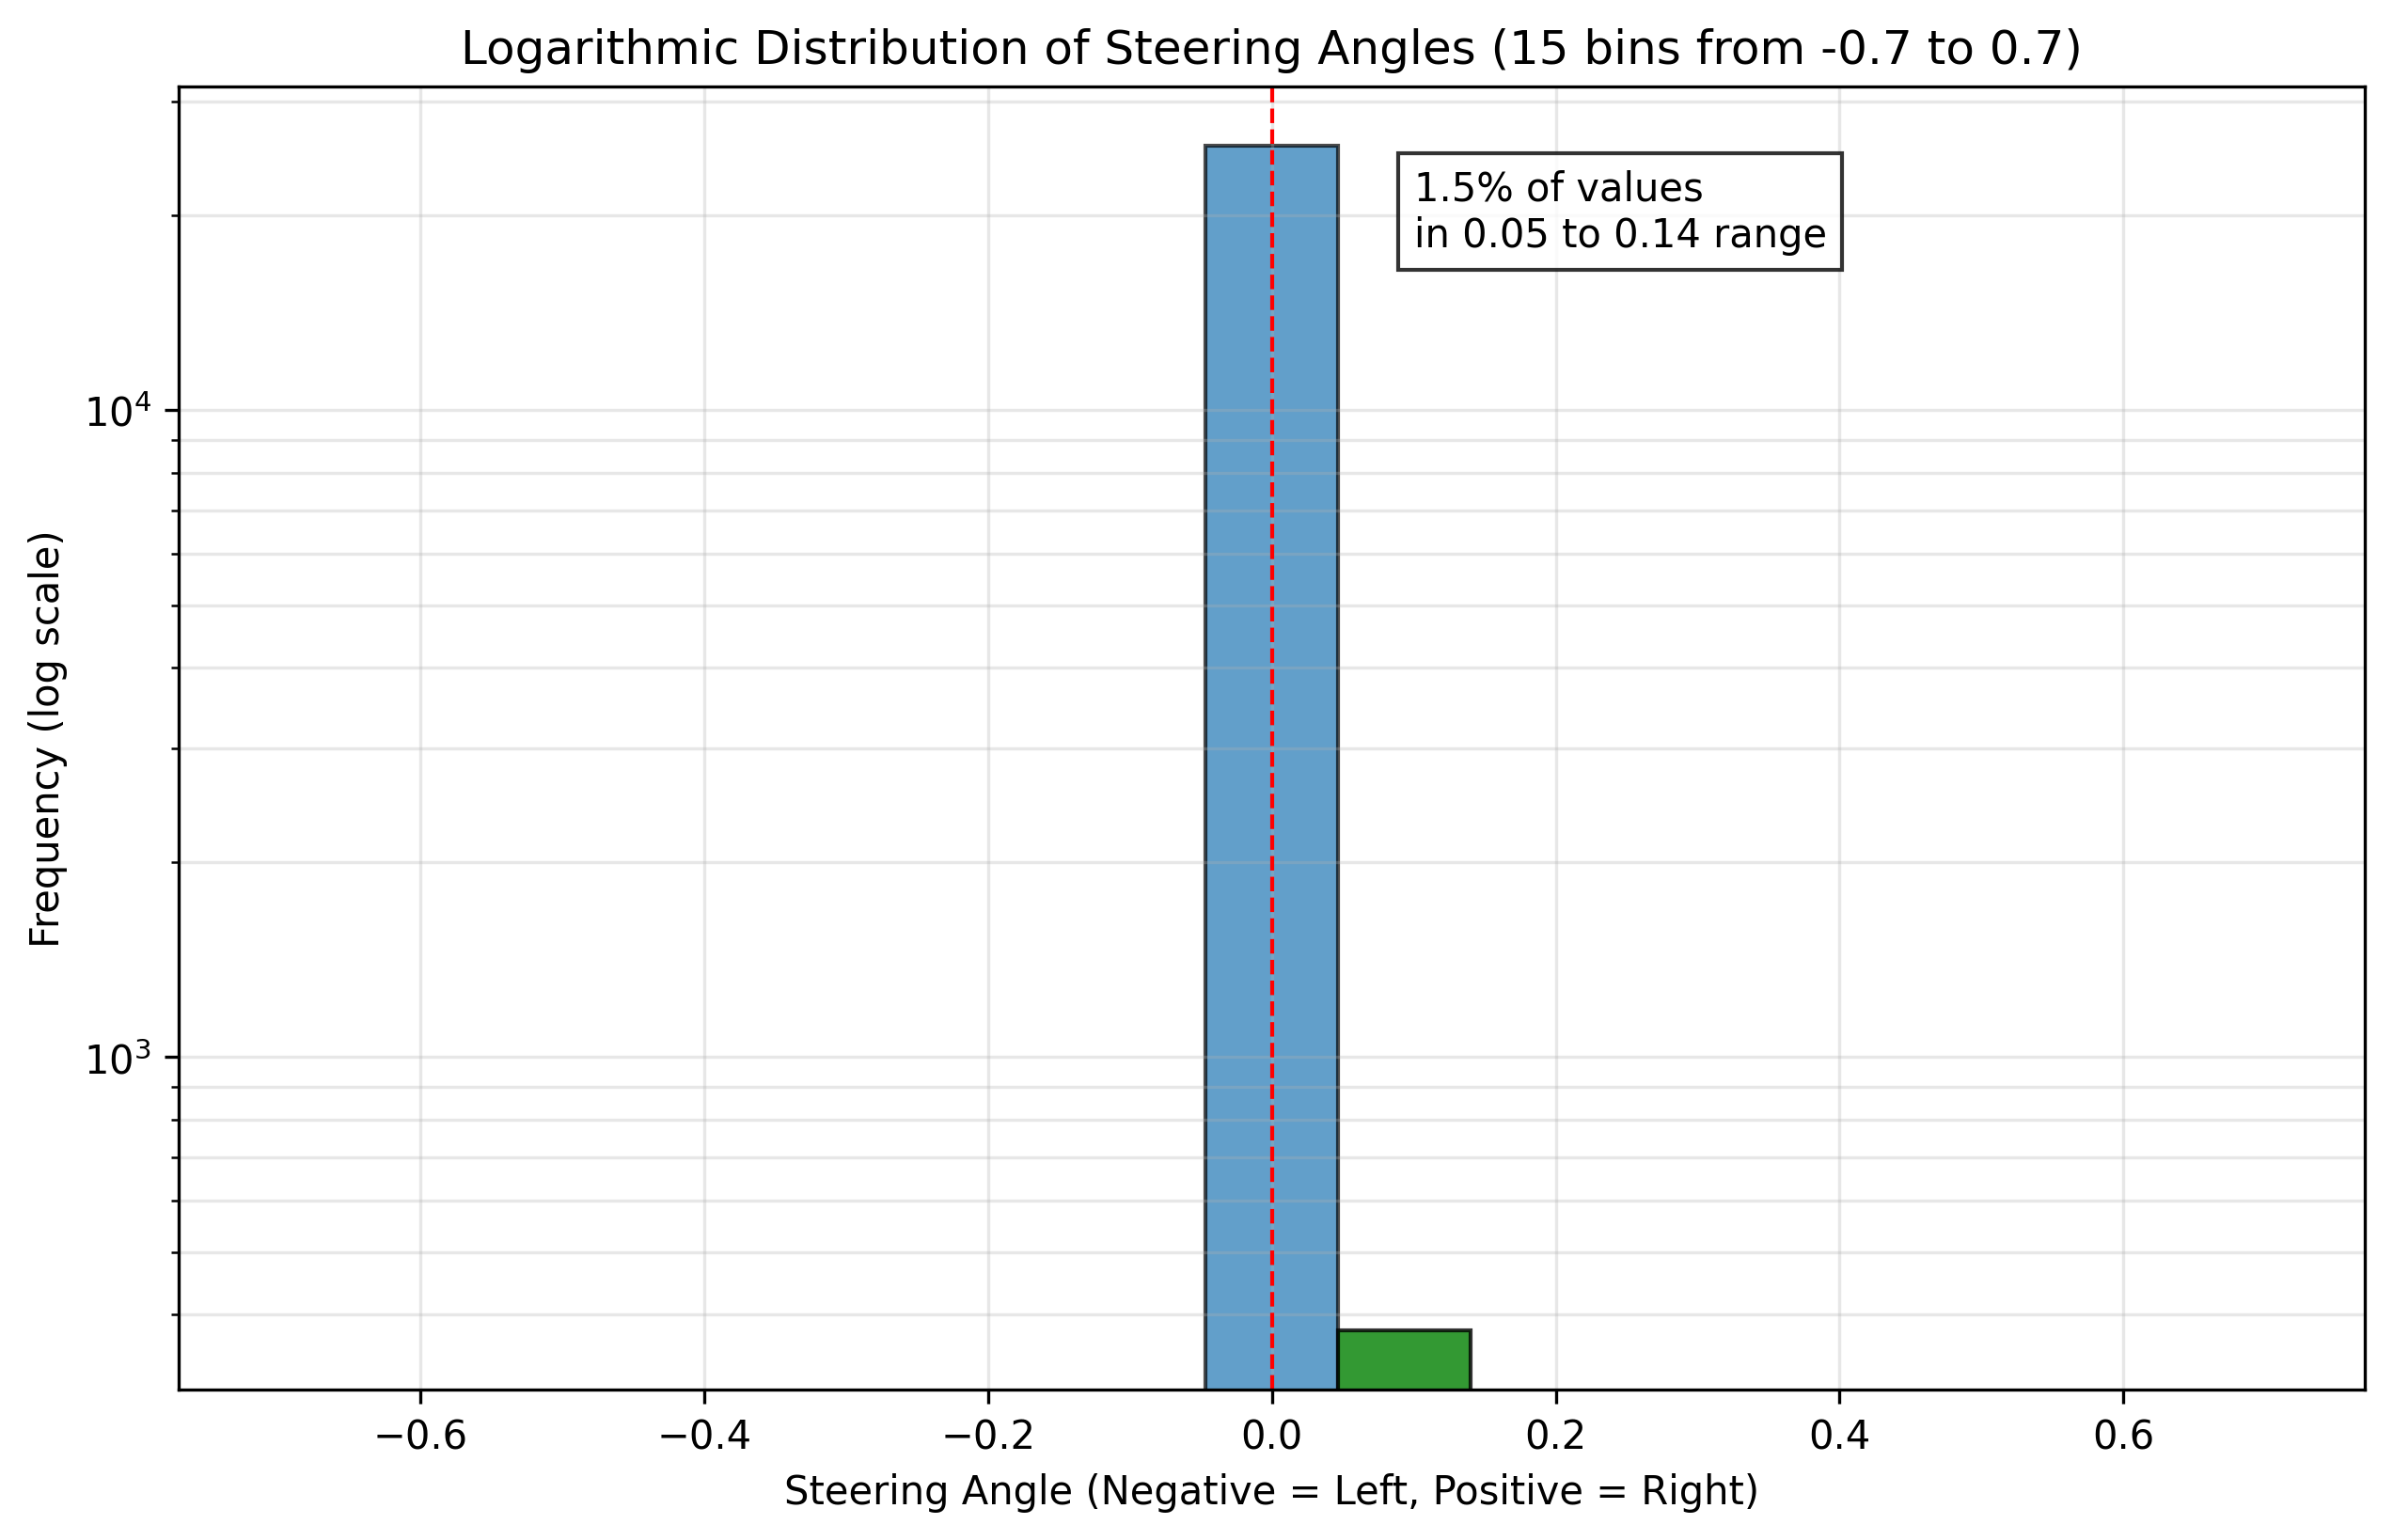
\includegraphics[width=0.99\textwidth]{Figures/Methods/steering_histogram_log.png}
    \caption{Ground truth steering around the entire figure 8 circuit (26k predictions histogram, Town04}
    \label{fig:/steering_histogram_log}
\end{figure}








